%% BlobFilters_manual.tex
%% natbib is loaded by tufte-book; force numerical citation style so that
%% a plain thebibliography environment is compatible.
\PassOptionsToPackage{numbers,sort&compress}{natbib}
%%
%% Manual for the BlobFilters MATLAB toolbox.
%% Typeset with the Tufte-LaTeX book class.
%%
%% Prerequisites
%%   tufte-latex  https://ctan.org/pkg/tufte-latex
%%   geometry, amsmath, booktabs, graphicx, listings, microtype,
%%   xcolor, hyperref  (all standard TeX Live / MiKTeX packages)
%%
%% Compile sequence (pdflatex + bibtex)
%%   pdflatex BlobFilters_manual
%%   bibtex   BlobFilters_manual
%%   pdflatex BlobFilters_manual
%%   pdflatex BlobFilters_manual
%%
%% Figures
%%   Generate all figure PDFs first by running docs/exportFigures.m in MATLAB.
%%   They are expected in docs/figures/ relative to this file.

\documentclass[a4paper, justified]{tufte-book}

% ---- packages ---------------------------------------------------------------
\usepackage{amsmath, amssymb}
\usepackage{booktabs}
\usepackage{graphicx}
\usepackage{microtype}
\usepackage{xcolor}
\usepackage{hyperref}
\usepackage{listings}
\usepackage{caption}

% ---- listings style (MATLAB) ------------------------------------------------
\definecolor{mComment}{rgb}{0.13,0.55,0.13}
\definecolor{mString} {rgb}{0.63,0.13,0.13}
\definecolor{mKeyword}{rgb}{0.00,0.00,1.00}

\lstdefinestyle{matlab}{
  language        = Matlab,
  basicstyle      = \small\ttfamily,
  keywordstyle    = \color{mKeyword}\bfseries,
  stringstyle     = \color{mString},
  commentstyle    = \color{mComment}\itshape,
  showstringspaces= false,
  breaklines      = true,
  frame           = single,
  framerule       = 0.4pt,
  backgroundcolor = \color{gray!8},
  numbers         = none,
  xleftmargin     = 6pt,
  xrightmargin    = 6pt,
}
\lstset{style=matlab}

% ---- Tufte tweaks -----------------------------------------------------------
\setcounter{secnumdepth}{2}
\setcounter{tocdepth}{1}
\hypersetup{colorlinks, linkcolor=blue!60!black, citecolor=green!40!black,
            urlcolor=blue!60!black}

% ---- title page -------------------------------------------------------------
\title{BlobFilters\\[0.5ex]
       \large A MATLAB Toolbox for Mitochondrial Structure Enhancement}
\author{Mark Fricker}
\date{March 2026 \quad\textbullet\quad Version 1.0}

% =============================================================================
\begin{document}
\maketitle
\tableofcontents

% =============================================================================
\chapter{Introduction}
\label{ch:intro}

\newthought{BlobFilters} is a MATLAB toolbox for enhancing elongated bright
structures---rods, fibres and tubular networks---against a noisy fluorescence
background. Its primary application is the detection and segmentation of
mitochondria in confocal images, where individual organelles appear as either
compact \emph{puncta} or elongated \emph{rods and networks} of approximately
8\,px width and 12--40\,px length.

The toolbox provides seven functions organised into three tiers:

\bigskip
\begin{tabular}{lp{0.55\linewidth}}
\toprule
\textbf{Tier} & \textbf{Functions} \\
\midrule
Blob / puncta detectors  & \texttt{logEnhance}, \texttt{granulometryEnhance} \\
Rod / fibre detectors    & \texttt{fiberEnhance}, \texttt{capsuleEnhance},
                           \texttt{rodGranulometryEnhance} \\
Orientation and pre-filtering
                         & \texttt{structureTensorEnhance},
                           \texttt{orientedGaussSmooth} \\
\bottomrule
\end{tabular}

\section{Quick start}

Add \texttt{src/} and \texttt{demos/} to the MATLAB path, then:

\begin{lstlisting}
addpath src demos

I = im2single(imread('my_confocal.tif'));

% Rod detector
pFib.widths  = [6 7 8 9 10];
R_fiber      = fiberEnhance(I, pFib);

% Rod granulometry
pRod.lengths = [8 12 16 20 28 36];
R_rod        = rodGranulometryEnhance(I, pRod);

% Structure tensor coherence as post-weight
pST.sigmaGrad = 1.5; pST.sigmaInt = 5;
C            = structureTensorEnhance(I, pST);
R_weighted   = R_rod .* C;    % suppress puncta
\end{lstlisting}

\section{Image conventions}

All functions accept any MATLAB numeric type and convert internally to
\texttt{single} in \([0,1]\) via \texttt{im2single}.  Inputs are expected to be
2-D (single-channel) grayscale images; passing an RGB array raises an error.

\section{Parameter defaults}

All parameters have sensible defaults tuned to 8\,px-wide, 12--40\,px-long
mitochondria imaged at typical confocal resolution.  Pass an empty struct or
omit the second argument to use defaults:
\begin{lstlisting}
R = fiberEnhance(I);           % use all defaults
R = fiberEnhance(I, struct()); % equivalent
\end{lstlisting}

% =============================================================================
\chapter{Blob and Puncta Detectors}
\label{ch:blobs}

% -----------------------------------------------------------------------------
\section{\texttt{logEnhance}}
\label{sec:log}

\newthought{The Laplacian-of-Gaussian} (LoG) is the canonical blob detector in
scale-space theory~\cite{Marr1980,Lindeberg1998}.  At scale $\sigma$ the
normalised LoG response is

\begin{equation}
  R_\sigma = -\sigma^2\,\nabla^2\bigl(G_\sigma * I\bigr),
  \label{eq:log}
\end{equation}

where $G_\sigma$ is a Gaussian with standard deviation $\sigma$ and
$\nabla^2 = \partial_{xx} + \partial_{yy}$ is the Laplacian.  The negative
sign gives a strong \emph{positive} response at bright circular blobs whose
characteristic radius is approximately $\sqrt{2}\,\sigma$.

\texttt{logEnhance} evaluates~\eqref{eq:log} at each requested scale and
returns the per-pixel maximum:

\begin{equation}
  R = \max_{\sigma \in \Sigma}\, R_\sigma.
\end{equation}

\subsection*{Separable implementation}

Rather than convolving directly with a 2-D LoG kernel, the image is first
smoothed by two 1-D Gaussian passes\sidenote{%
  \texttt{imfilter} requires the kernel to be of class \texttt{double}
  regardless of the image class; both the 1-D Gaussian and the Laplacian are
  kept as \texttt{double}.}
and then filtered with the compact $3\times3$ discrete Laplacian
$\ell = [0,1,0;\,1,-4,1;\,0,1,0]$.  This reduces the per-scale cost from
$O(N^2(6\sigma)^2)$ to $O(N^2 \cdot 6\sigma)$, approximately a $6\times$
speedup at $\sigma=6$.

\subsection*{Parameters}
\marginnote{%
  \textbf{\texttt{sigmas}} \newline
  Vector of $\sigma$ values (px). Default \texttt{[2 3 4 5 6]}.\newline
  Rule of thumb: $\sigma \approx r/\sqrt{2}$ for a blob of radius $r$.
  \medskip\par
  \textbf{\texttt{normalize}} \newline
  Rescale output to $[0,1]$. Default \texttt{true}.
}

\begin{lstlisting}
pLog.sigmas    = [2 3 4 5 6];   % sigma ~ radius/sqrt(2)
pLog.normalize = true;
R = logEnhance(I, pLog);
\end{lstlisting}

% -----------------------------------------------------------------------------
\section{\texttt{granulometryEnhance}}
\label{sec:gran}

\newthought{Granulometry} characterises the size distribution of bright objects
via the \emph{pattern spectrum}~\cite{Maragos1989,Serra1982}.  A morphological
opening with a disk of radius $r$ removes all bright structures narrower than
$2r$; the residue

\begin{equation}
  \mathrm{PS}(r) = \mathrm{Open}(I, \mathrm{disk}(r))
                 - \mathrm{Open}(I, \mathrm{disk}(r{+}\Delta r))
\end{equation}

is large wherever structures of scale $r$ exist.  Summing over all consecutive
radius pairs yields an integrated enhancement map that highlights objects across
all specified scales.

Disk openings are \emph{isotropic}: compact puncta and short rods at the same
scale both respond.  Multiplying the output by the structure tensor coherence
$C$ (Section~\ref{sec:st}) suppresses round puncta.

\subsection*{Parameters}
\marginnote{%
  \textbf{\texttt{sigmas}} \newline
  Disk radii (px). Default \texttt{[1 2 3 4 8 16 32]}.\newline
  At least 2 values are required.
  \medskip\par
  \textbf{\texttt{normalize}} \newline
  Default \texttt{true}.
}

\begin{lstlisting}
pGran.sigmas    = [2 4 6 8 10 12 16];
pGran.normalize = true;
G = granulometryEnhance(I, pGran);
\end{lstlisting}

% =============================================================================
\chapter{Rod and Fibre Detectors}
\label{ch:rods}

% -----------------------------------------------------------------------------
\section{\texttt{fiberEnhance}}
\label{sec:fiber}

\newthought{fiberEnhance} wraps the MATLAB Image Processing Toolbox function
\texttt{fibermetric}, which implements a Frangi-style tubularity
measure~\cite{Frangi1998}.  At each scale $w$ the Hessian of the
Gaussian-smoothed image is computed; for a bright tubular ridge the smaller
eigenvalue $\lambda_1$ is large and negative while $\lambda_2 \approx 0$.  The
per-pixel response is

\begin{equation}
  S_w = e^{-\lambda_1}\bigl(1 - e^{\lambda_2/c}\bigr),
\end{equation}

where $c$ is an automatic scale factor.  \texttt{fibermetric} aggregates over
all widths and selects the best-scale response per pixel.

\subsection*{Multimode options}

\begin{description}
  \item[\texttt{'builtin'}] (default) Passes all widths to \texttt{fibermetric}
    at once; MathWorks selects the best scale per pixel.
  \item[\texttt{'stack'}] Calls \texttt{fibermetric} once per width and takes
    the pixel-wise maximum---useful for inspecting individual scale responses.
\end{description}

\subsection*{Parameters}
\marginnote{%
  \textbf{\texttt{widths}} \newline
  Cross-sectional widths (px). Default \texttt{[6 7 8 9 10]}.\newline
  Probe the \emph{short axis} only; length is not a parameter.
  \medskip\par
  \textbf{\texttt{multimode}} \newline
  \texttt{'builtin'} or \texttt{'stack'}. Default \texttt{'builtin'}.
  \medskip\par
  Requires IPT R2018b+.
}

\begin{lstlisting}
pFib.widths    = [6 7 8 9 10];
pFib.multimode = 'builtin';
pFib.normalize = true;
R = fiberEnhance(I, pFib);
\end{lstlisting}

% -----------------------------------------------------------------------------
\section{\texttt{capsuleEnhance}}
\label{sec:capsule}

\newthought{Capsule kernels} are oriented templates shaped like a
stadium\sidenote{%
  A \emph{stadium} (or \emph{discorectangle}) is a rectangle capped by two
  half-disks of the same radius.  Also known as an oblong or a capsule.}---a
rectangle capped with two semicircles---that match the cross-sectional profile
of a mitochondrion.  A bank of kernels at different lengths and orientations
is convolved with the image, and the per-pixel maximum response over the bank
is returned.

Two kernel modes are available:
\begin{description}
  \item[\texttt{'single'}] Normalised positive capsule kernel.  Gives high
    response wherever a bright rod matches the kernel footprint.
  \item[\texttt{'doc'}] Difference-of-Capsules (DoC): the response of a narrow
    inner capsule minus $\alpha$ times a wider inhibitory surround.  Suppresses
    signal from clustered or touching mitochondria.
\end{description}

Kernels are unit-sum-normalised after mean subtraction so that a flat background
gives zero response.

\subsection*{Parameters}
\marginnote{%
  \textbf{\texttt{lengths}} \newline
  Capsule body lengths (px). Default \texttt{[12 16 20 28 36 40]}.
  \medskip\par
  \textbf{\texttt{width}} \newline
  Capsule half-width / end radius (px). Default \texttt{8}.
  \medskip\par
  \textbf{\texttt{wideWidth}} \newline
  DoC outer radius (px). Default \texttt{16}.
  \medskip\par
  \textbf{\texttt{alpha}} \newline
  DoC inhibitory weight $\in(0,1)$. Default \texttt{0.5}.
  \medskip\par
  \textbf{\texttt{orientations}} \newline
  Number of angles in $[0^\circ,180^\circ)$. Default \texttt{12}.
  \medskip\par
  \textbf{\texttt{mode}} \newline
  \texttt{'single'} or \texttt{'doc'}. Default \texttt{'single'}.
}

\begin{lstlisting}
% Single mode
pCapS.lengths      = [12 16 20 28 36 40];
pCapS.width        = 8;
pCapS.orientations = 12;
pCapS.mode         = 'single';
R_single = capsuleEnhance(I, pCapS);

% DoC mode
pCapD.wideWidth = 18; pCapD.alpha = 0.55;
pCapD.mode      = 'doc';
R_doc = capsuleEnhance(I, pCapD);
\end{lstlisting}

% -----------------------------------------------------------------------------
\section{\texttt{rodGranulometryEnhance}}
\label{sec:rodgran}

\newthought{Rod granulometry} replaces the isotropic disk SE of
\texttt{granulometryEnhance} with a bank of oriented line structuring
elements~\cite{Soille2003}.  At each length $L$ the maximum opening over all
orientations $\theta$ is computed:

\begin{equation}
  O_{\max}(L) = \max_{\theta}\,\mathrm{Open}\!\left(I,\,
                 \mathrm{line}(L, \theta)\right),
\end{equation}

and the pattern spectrum residue $O_{\max}(L_k) - O_{\max}(L_{k+1})$ isolates
structures of length approximately $L_k$ pixels.

Because a compact punctum cannot survive a line opening longer than its own
diameter, line SEs are \emph{inherently} selective for elongated structures
without needing coherence post-weighting---a key advantage over disk
granulometry.

\subsection*{Parameters}
\marginnote{%
  \textbf{\texttt{lengths}} \newline
  Line lengths (px). Default \texttt{[8 12 16 20 28 36]}.\newline
  Rod of length $L_\text{rod}$ responds at the largest $L_k < L_\text{rod}$.
  \medskip\par
  \textbf{\texttt{orientations}} \newline
  Number of angles in $[0^\circ,180^\circ)$. Default \texttt{8}.
  \medskip\par
  \textbf{\texttt{normalize}} Default \texttt{true}.
}

\begin{lstlisting}
pRod.lengths      = [8 12 16 20 28 36];
pRod.orientations = 8;
R = rodGranulometryEnhance(I, pRod);
\end{lstlisting}

% -----------------------------------------------------------------------------
\section{\texttt{cellposeEnhance}}
\label{sec:cellpose}

\newthought{cellposeEnhance} wraps the MathWorks Medical Imaging Toolbox
Interface for Cellpose Library~\cite{Stringer2021,Stringer2025}, providing
deep-learning cell segmentation from within MATLAB.

Unlike the other BlobFilters enhancers, which return continuous probability-like
maps, \texttt{cellposeEnhance} returns a \emph{binary} mask and an integer label
image:

\begin{description}
  \item[\texttt{R}] Binary single $\{0,1\}$ mask compatible with the $[0,1]$
    convention of every other enhancer.  Can be used as a multiplicative weight,
    a seed mask, or a segmentation result directly.
  \item[\texttt{L}] \texttt{uint16} label image.  Each detected object carries
    a unique positive integer; background is~0.  Neighbouring or touching objects
    that would merge under simple thresholding are distinguished here.
\end{description}

\begin{lstlisting}
[R, L] = cellposeEnhance(I);           % defaults: cyto3, diameter 10 px
imshow(label2rgb(L, 'hsv', 'k'))       % coloured instance map
\end{lstlisting}

\subsection*{Parameters}
\marginnote{%
  \textbf{\texttt{model}} \newline
  Cellpose model name or path to a custom model file.
  Default \texttt{'cyto3'}.
  \medskip\par
  \textbf{\texttt{diameter}} \newline
  Expected object cross-section (px). Default \texttt{10}.\newline
  Set to \texttt{0} for automatic estimation (slower).
  \medskip\par
  Requires the \emph{Medical Imaging Toolbox Interface for Cellpose Library}
  add-on and a Python environment with \texttt{cellpose} installed.
}

\subsection*{Model choice for mitochondria}

The \texttt{'cyto3'} model (Cellpose~3, Nature Methods 2025) is a suitable
default for fluorescence mitochondria images: it was trained on nine
heterogeneous datasets and generalises well to sub-cellular structures.  For
higher specificity, fine-tune a custom model with 100--200 manually annotated
frames using the Cellpose~2.0 human-in-the-loop GUI, then supply the saved
model path:

\begin{lstlisting}
pCP.model    = 'C:\models\mito_finetuned';
pCP.diameter = 10;
[R, L] = cellposeEnhance(I, pCP);
\end{lstlisting}

\subsection*{Parameter optimisation for mitochondria fluorescence}
\label{sec:cellpose-sweep}

\newthought{A systematic sweep} of \texttt{cellProb} and
\texttt{flowThreshold} was carried out using the companion script
\texttt{sweepCellpose.m} (located in
\texttt{Segmentation\_sandbox/demos/}) on a cropped fluorescence
mitochondria image (\texttt{mitImagecrop.mat}, same field of view used
throughout).  Two additional axes were explored: the specialised
\texttt{bact\_fluor\_cp3} model (Cellpose~3, trained on fluorescent
bacteria whose morphology resembles elongated mitochondria) and an
increased iteration count (\texttt{nIter}~=~2000, recommended in the
literature for long thin structures~\cite{Stringer2025}).

\medskip
\noindent\textbf{Parameters swept.}
\marginnote{%
  \textbf{Metrics} \\
  \textit{n objects}: number of distinct detected objects
  (\texttt{max(L(:))}); too high indicates over-segmentation or noise
  detections. \\[4pt]
  \textit{coverage\,\%}: fraction of image pixels labelled as
  foreground; should match the expected mitochondrial area fraction.
}
\begin{itemize}
  \item \texttt{cellProb} (\texttt{CellThreshold}): broad survey
        $[-4, \ldots, +2]$, narrowed to $[-2, -1, 0, +1]$, then
        finalised at $[-1, 0, +1]$.
  \item \texttt{flowThreshold} (\texttt{FlowErrorThreshold}): $[0.30,
        0.50, 0.80, 1.20]$, finalised at $[0.60, 0.80, 1.00]$.
  \item Models: \texttt{cyto3} and \texttt{bact\_fluor\_cp3}.
  \item \texttt{nIter}: $0$ (default $\approx$200) and $2000$.
\end{itemize}

\noindent\textbf{Findings.}
\begin{itemize}
  \item \texttt{bact\_fluor\_cp3} produced over-segmentation on this
        image and performed worse than \texttt{cyto3} across all
        parameter combinations.
  \item Increasing \texttt{nIter} to 2000 gave no improvement in object
        count, coverage, or visual boundary quality for
        \texttt{cyto3}.
  \item The useful operating region for \texttt{cyto3} was
        $\mathtt{cellProb} \in [-1, 0]$ combined with
        $\mathtt{flowThreshold} \in [0.8, 1.2]$.  Outside this region
        object counts increased sharply (over-segmentation) or dropped
        steeply (under-detection).
  \item $\mathtt{cellProb} = 0$ produced visually tighter outlines that
        better matched individual mitochondria compared with the more
        permissive $-1$.
\end{itemize}

\noindent\textbf{Recommended settings} (used as ground truth in
\texttt{sweepSegmentation.m}):

\begin{lstlisting}
pCP.model         = 'cyto3';
pCP.diameter      = 10;      % px - typical mitochondrion cross-section
pCP.cellProb      = 0;       % CellThreshold; lower = more sensitive
pCP.flowThreshold = 0.8;     % FlowErrorThreshold
[R, L] = cellposeEnhance(I, pCP);
\end{lstlisting}

% --- cyto3, default nIter ------------------------------------------------
\IfFileExists{figures/cellpose_sweep_heatmaps_cyto3.pdf}{%
\begin{figure*}
  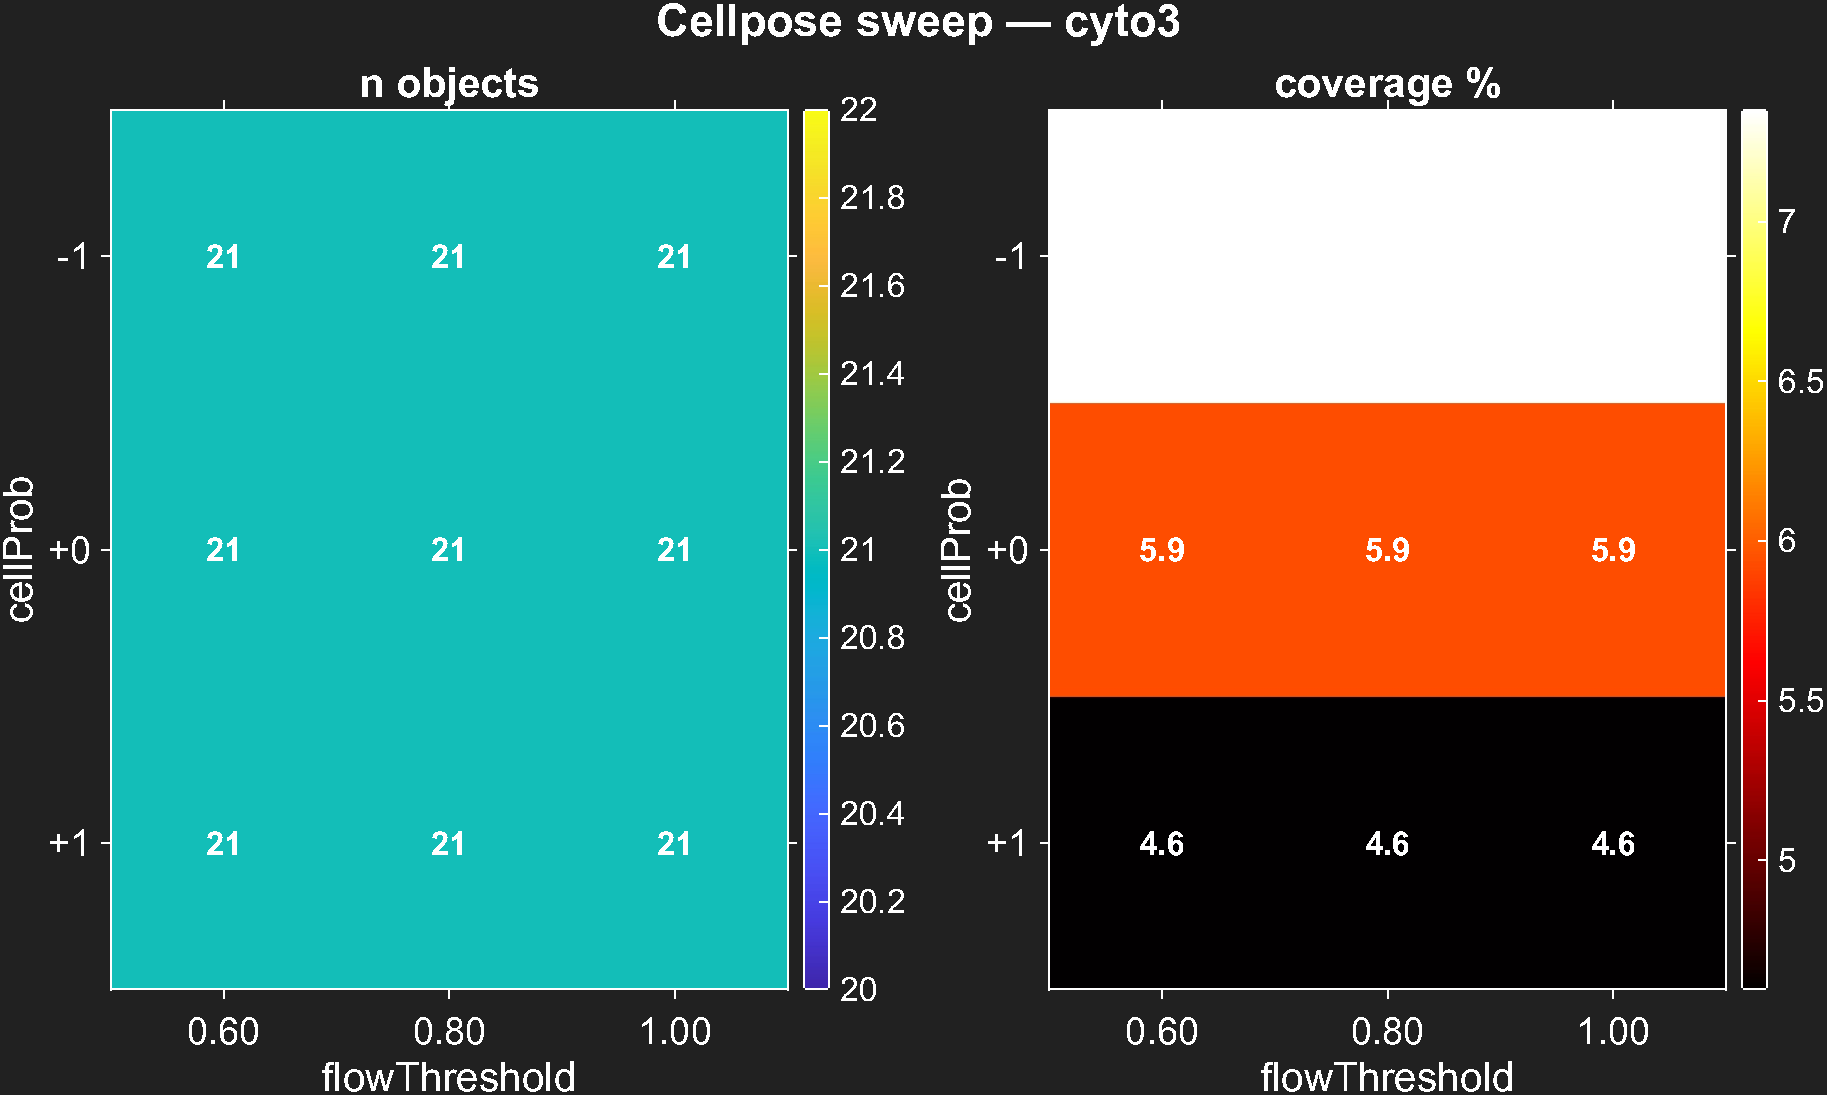
\includegraphics[width=\linewidth]{figures/cellpose_sweep_heatmaps_cyto3.pdf}
  \caption{\texttt{cyto3} sweep heatmaps (default \texttt{nIter}).
    Left: number of detected objects.  Right: foreground coverage~(\%).
    Rows = \texttt{cellProb} $\in \{-1, 0, +1\}$;
    columns = \texttt{flowThreshold} $\in \{0.60, 0.80, 1.00\}$.
    The cell at $\mathtt{cellProb}=0$, $\mathtt{flowThreshold}=0.8$ gives
    the best balance of object count and boundary tightness.}
  \label{fig:cellpose-cyto3-heatmaps}
\end{figure*}
}{%
\begin{quote}\textit{Run \texttt{sweepCellpose.m} with \texttt{doExport = true}
  to generate \texttt{cellpose\_sweep\_heatmaps\_cyto3.pdf}.}\end{quote}
}

\IfFileExists{figures/cellpose_sweep_labels_cyto3.pdf}{%
\begin{figure*}
  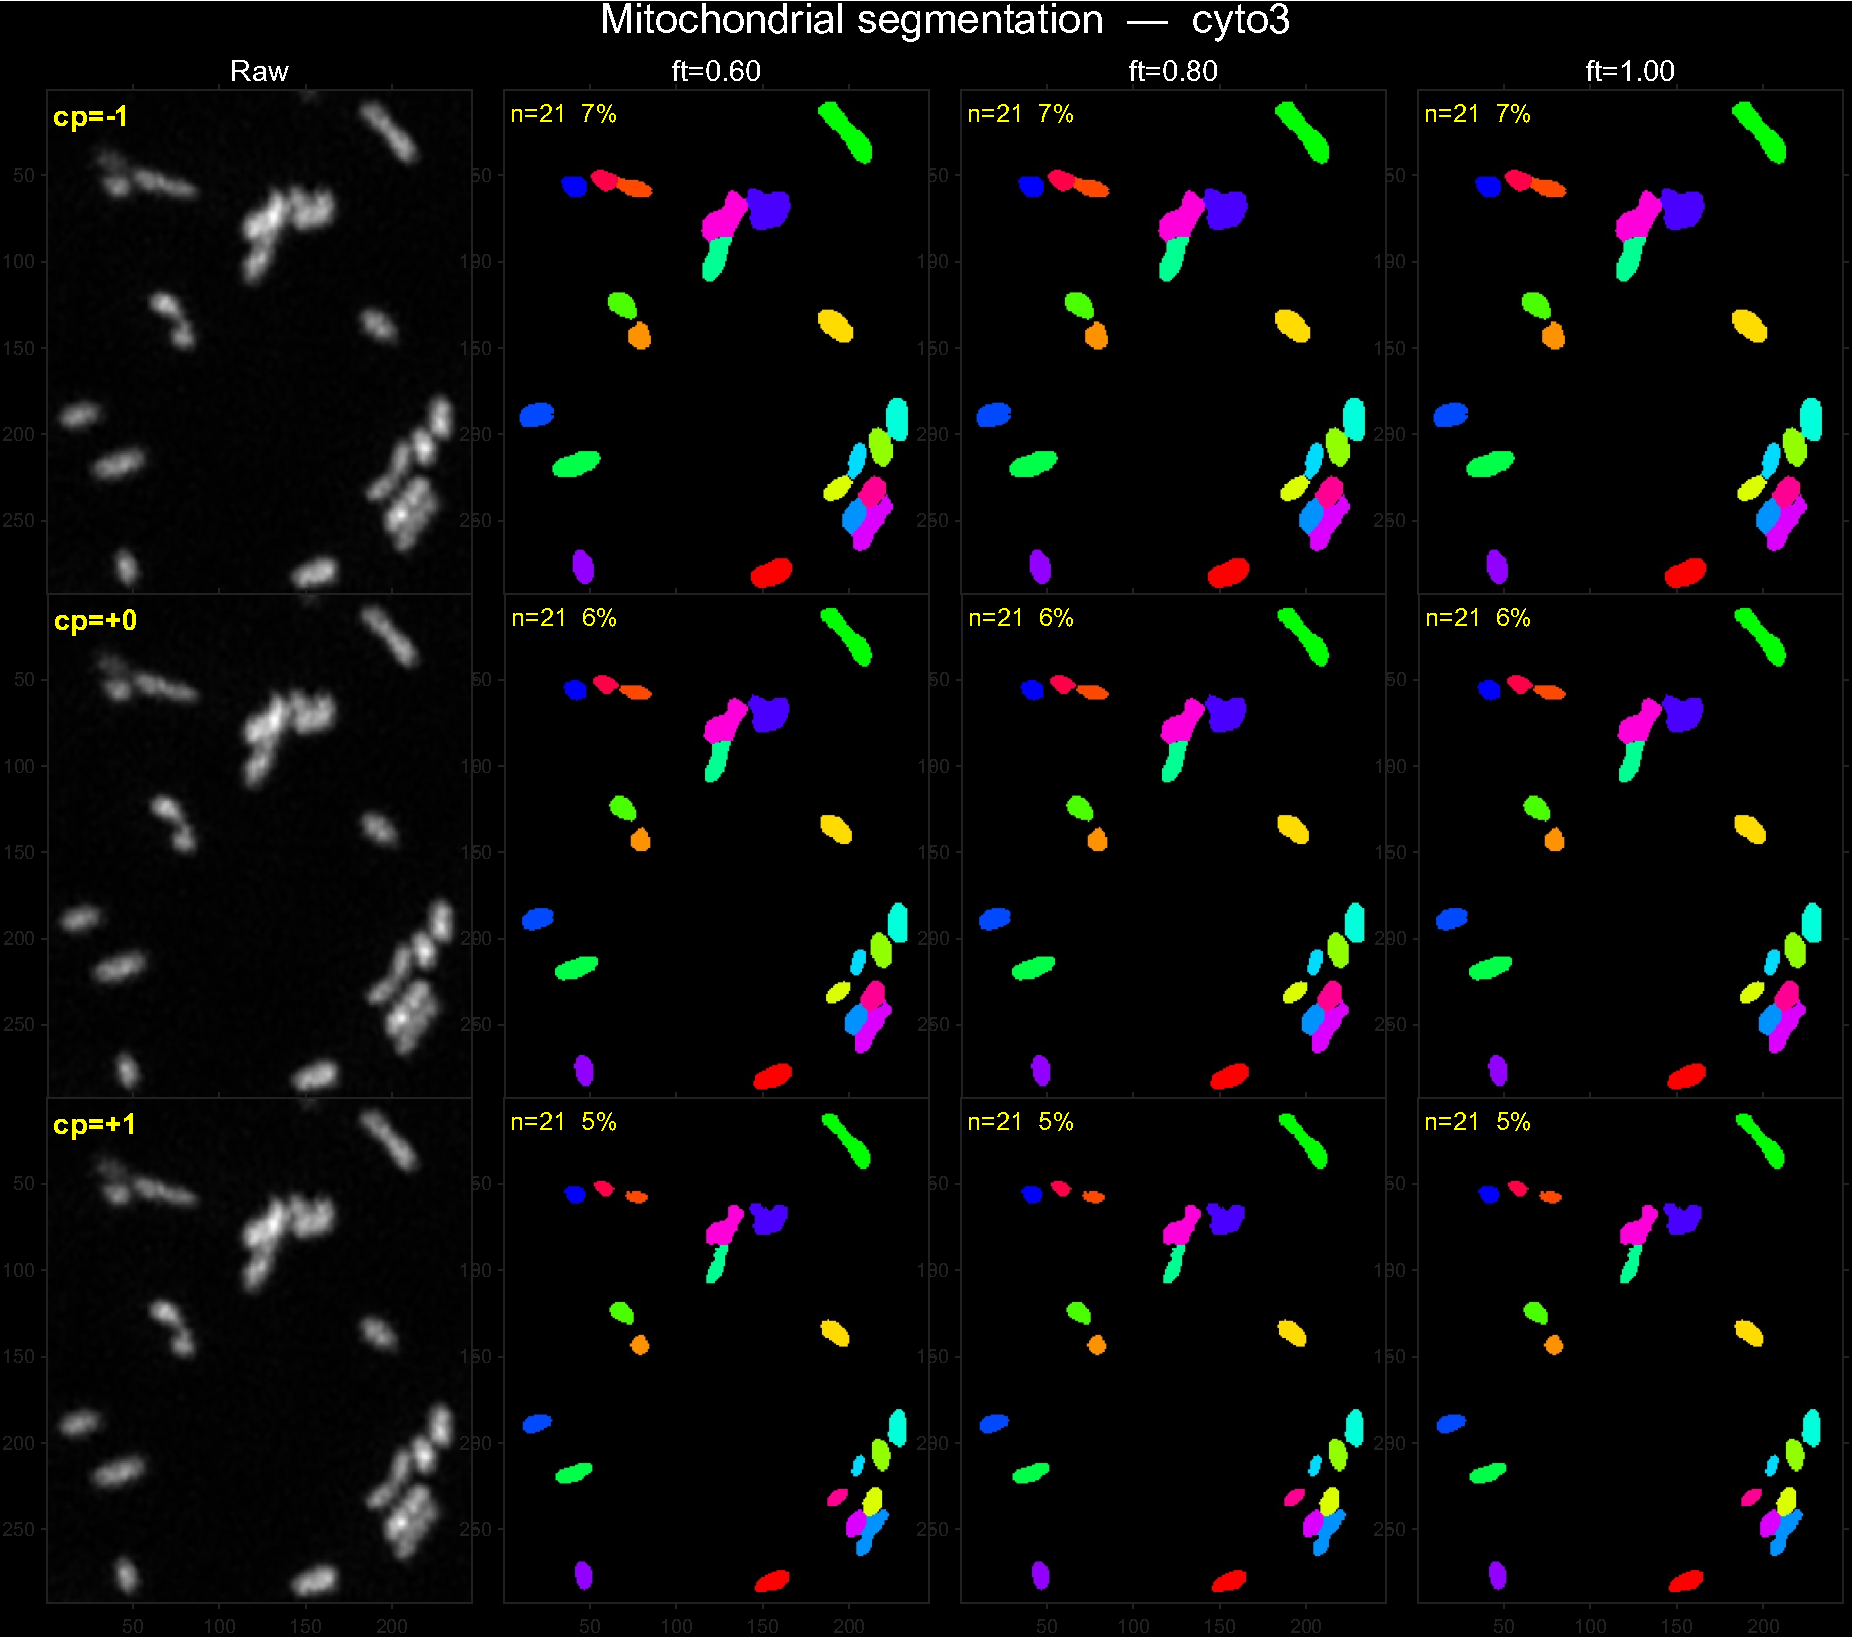
\includegraphics[width=\linewidth]{figures/cellpose_sweep_labels_cyto3.pdf}
  \caption{\texttt{cyto3} label grid (default \texttt{nIter}).
    Rows = \texttt{cellProb} ($-1$, $0$, $+1$).  Column~1: raw image.
    Columns 2--4: instance labels (\texttt{label2rgb}) for
    \texttt{flowThreshold} $= 0.60$, $0.80$, $1.00$.
    Black pixels are background.}
  \label{fig:cellpose-cyto3-labels}
\end{figure*}
}{%
\begin{quote}\textit{Run \texttt{sweepCellpose.m} with \texttt{doExport = true}
  to generate \texttt{cellpose\_sweep\_labels\_cyto3.pdf}.}\end{quote}
}

% --- cyto3, nIter = 2000 -------------------------------------------------
\IfFileExists{figures/cellpose_sweep_heatmaps_cyto3_nIter-2000.pdf}{%
\begin{figure*}
  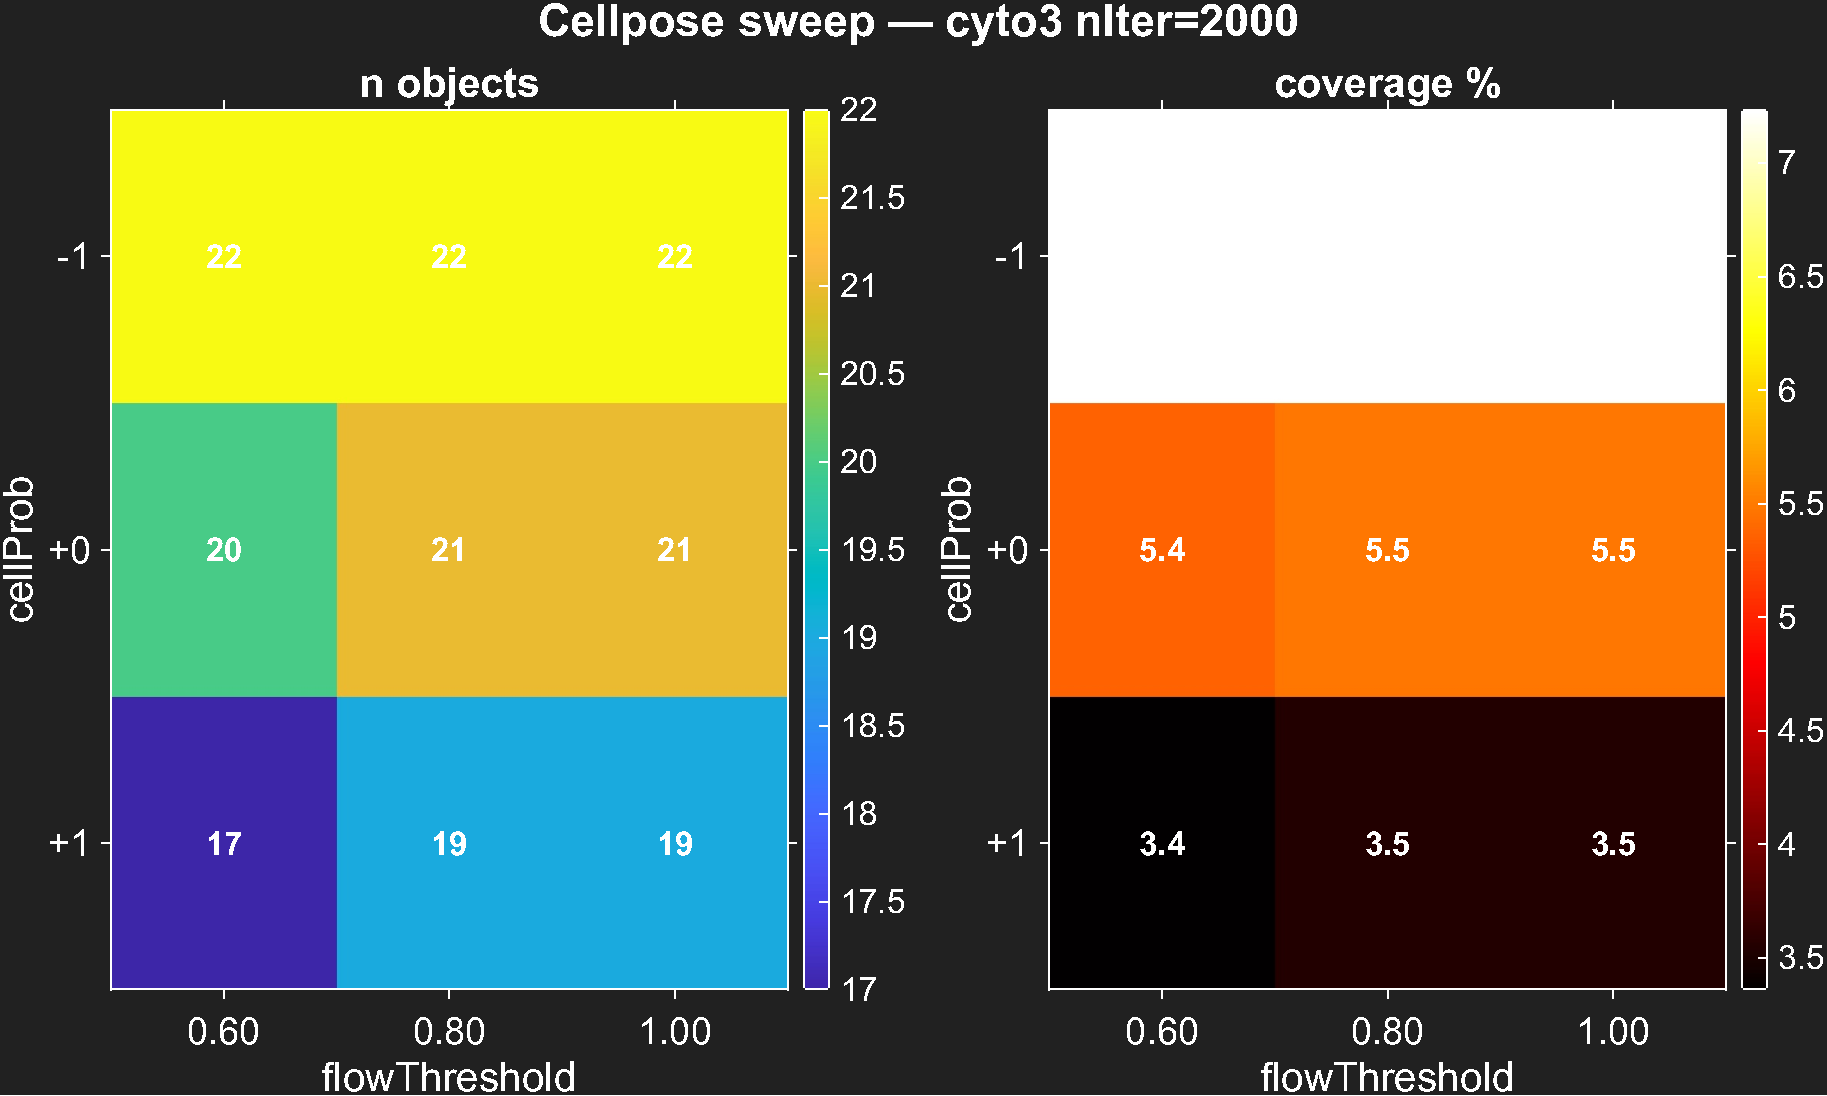
\includegraphics[width=\linewidth]{figures/cellpose_sweep_heatmaps_cyto3_nIter-2000.pdf}
  \caption{\texttt{cyto3} sweep heatmaps with \texttt{nIter}~=~2000.
    Layout as Figure~\ref{fig:cellpose-cyto3-heatmaps}.
    Compare with the default-\texttt{nIter} result to assess whether
    additional iterations alter object count or coverage.}
  \label{fig:cellpose-cyto3-niter-heatmaps}
\end{figure*}
}{%
\begin{quote}\textit{Run \texttt{sweepCellpose.m} with \texttt{doExport = true}
  to generate \texttt{cellpose\_sweep\_heatmaps\_cyto3\_nIter-2000.pdf}.}\end{quote}
}

\IfFileExists{figures/cellpose_sweep_labels_cyto3_nIter-2000.pdf}{%
\begin{figure*}
  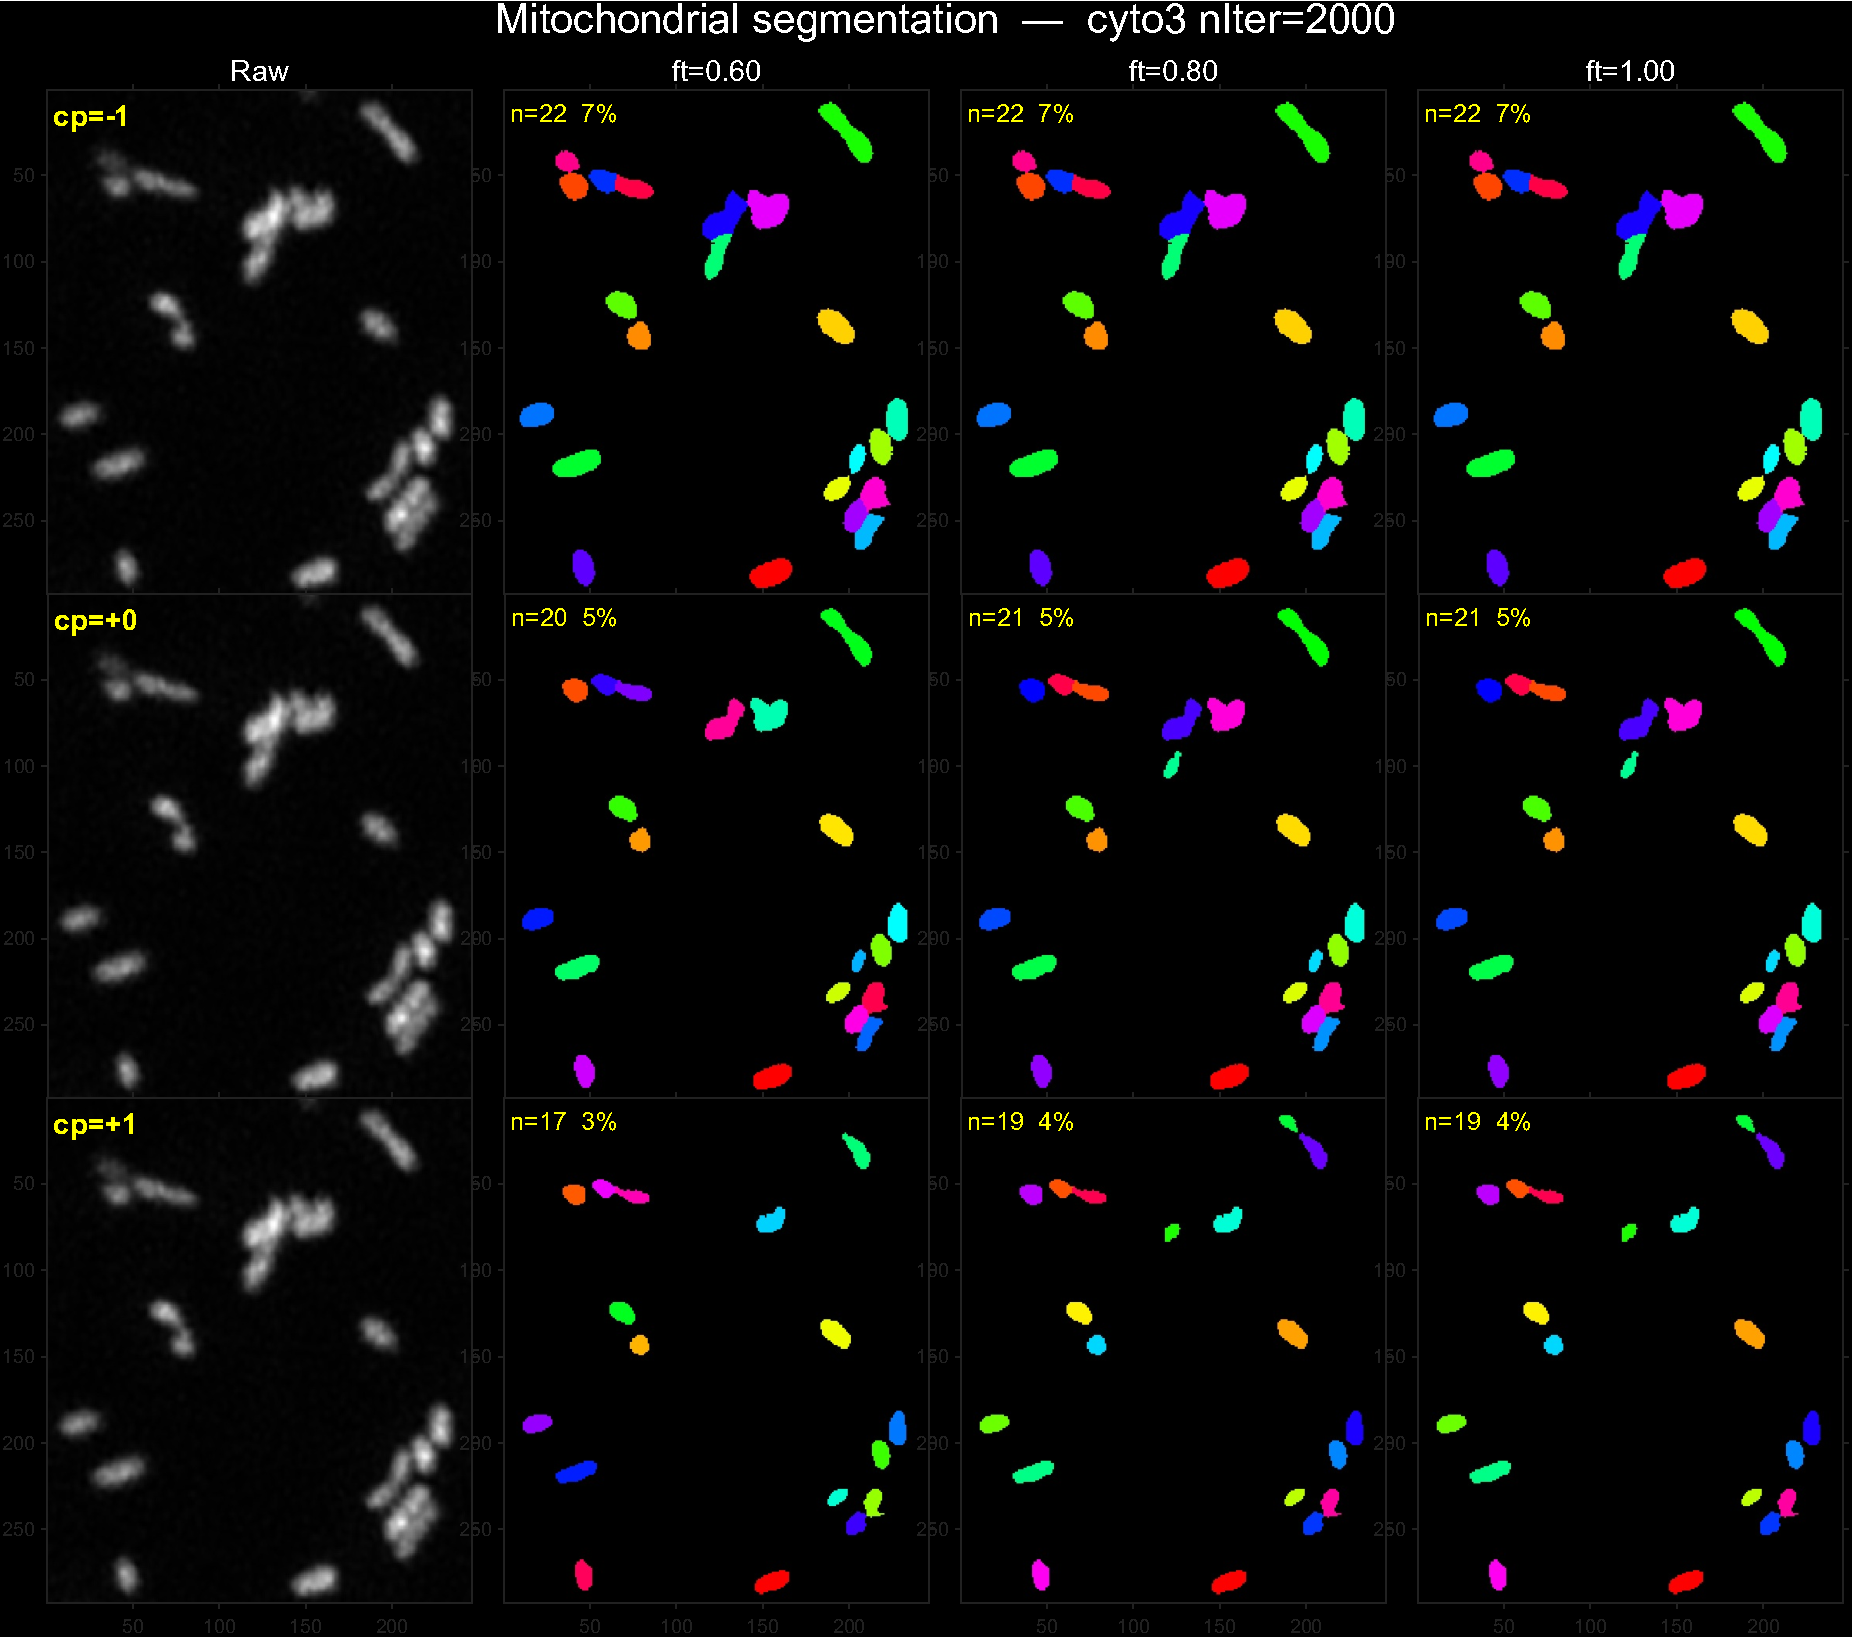
\includegraphics[width=\linewidth]{figures/cellpose_sweep_labels_cyto3_nIter-2000.pdf}
  \caption{\texttt{cyto3} label grid with \texttt{nIter}~=~2000.
    Layout as Figure~\ref{fig:cellpose-cyto3-labels}.}
  \label{fig:cellpose-cyto3-niter-labels}
\end{figure*}
}{%
\begin{quote}\textit{Run \texttt{sweepCellpose.m} with \texttt{doExport = true}
  to generate \texttt{cellpose\_sweep\_labels\_cyto3\_nIter-2000.pdf}.}\end{quote}
}

% --- bact\_fluor\_cp3, default nIter -------------------------------------
\IfFileExists{figures/cellpose_sweep_heatmaps_bact_fluor_cp3.pdf}{%
\begin{figure*}
  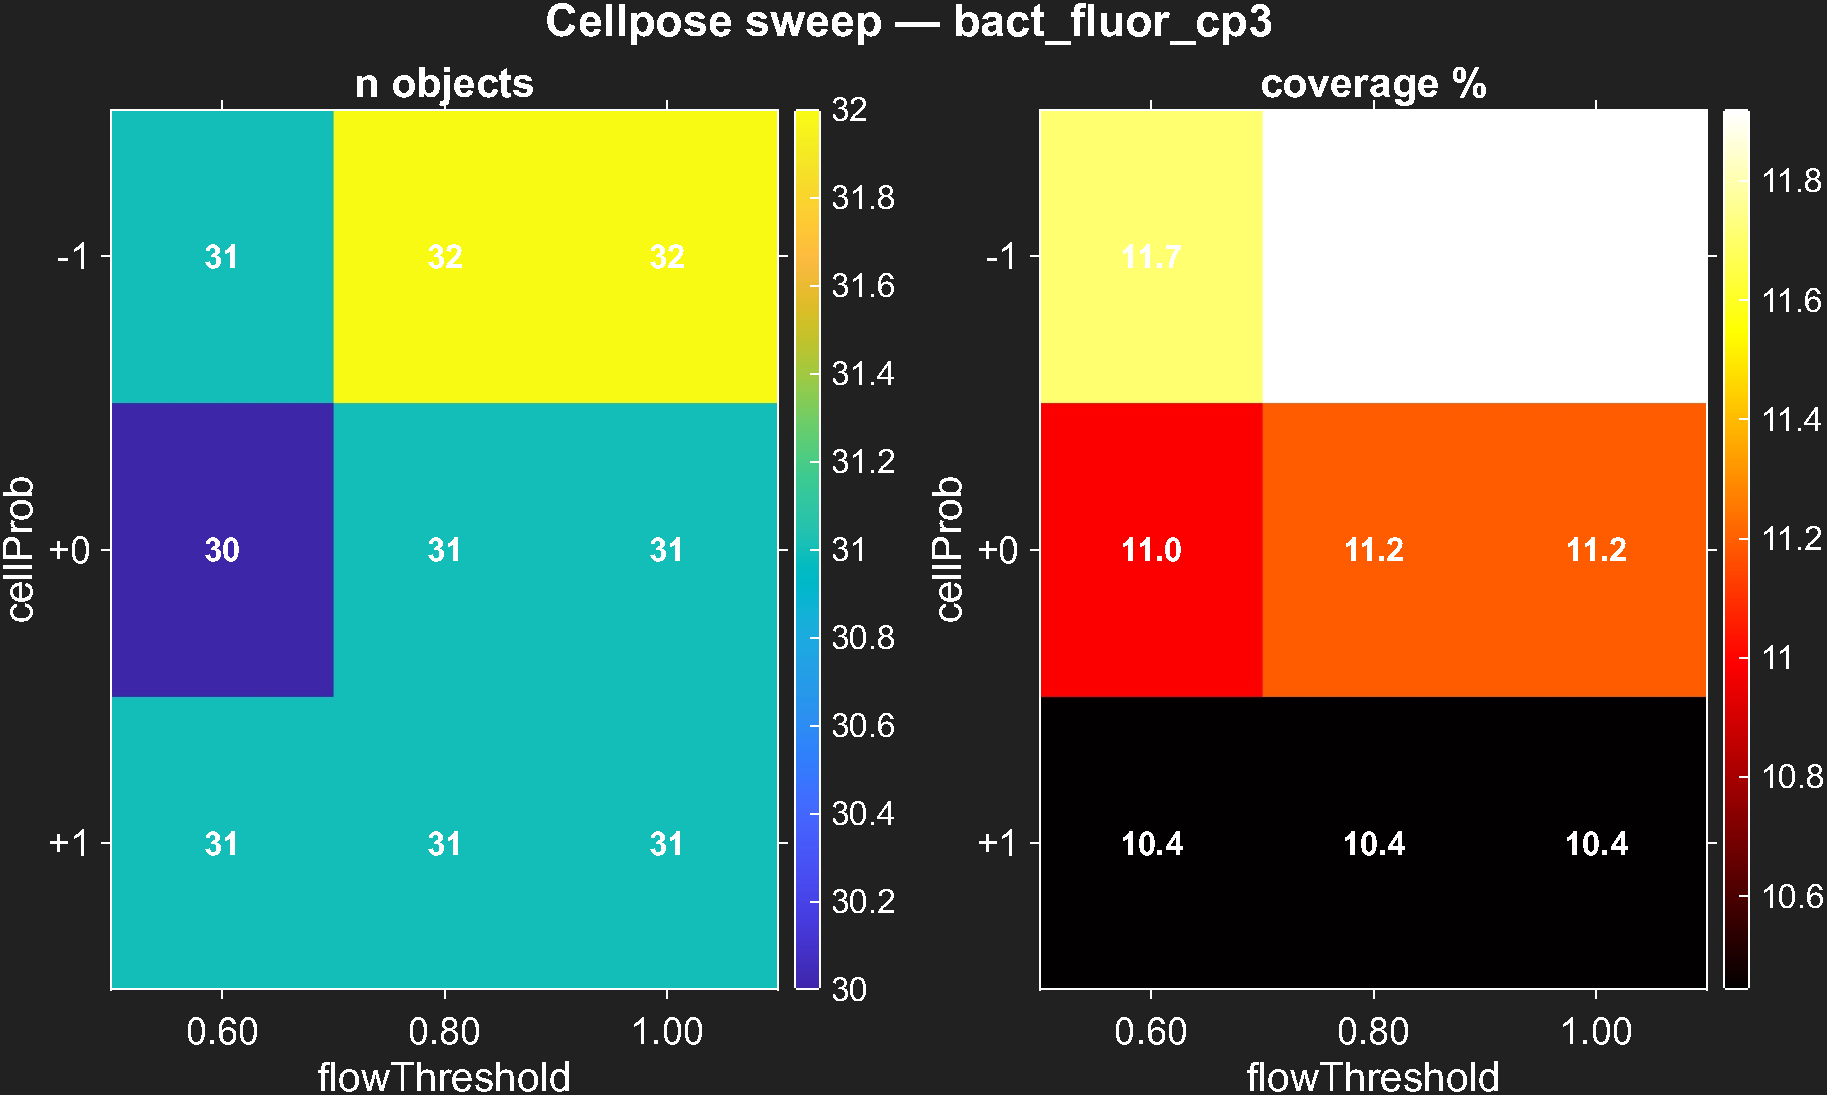
\includegraphics[width=\linewidth]{figures/cellpose_sweep_heatmaps_bact_fluor_cp3.pdf}
  \caption{\texttt{bact\_fluor\_cp3} sweep heatmaps (default \texttt{nIter}).
    Layout as Figure~\ref{fig:cellpose-cyto3-heatmaps}.
    This model is trained on fluorescent bacteria; compare object counts
    and coverage with the \texttt{cyto3} results above.}
  \label{fig:cellpose-bact-heatmaps}
\end{figure*}
}{%
\begin{quote}\textit{Run \texttt{sweepCellpose.m} with \texttt{doExport = true}
  to generate \texttt{cellpose\_sweep\_heatmaps\_bact\_fluor\_cp3.pdf}.}\end{quote}
}

\IfFileExists{figures/cellpose_sweep_labels_bact_fluor_cp3.pdf}{%
\begin{figure*}
  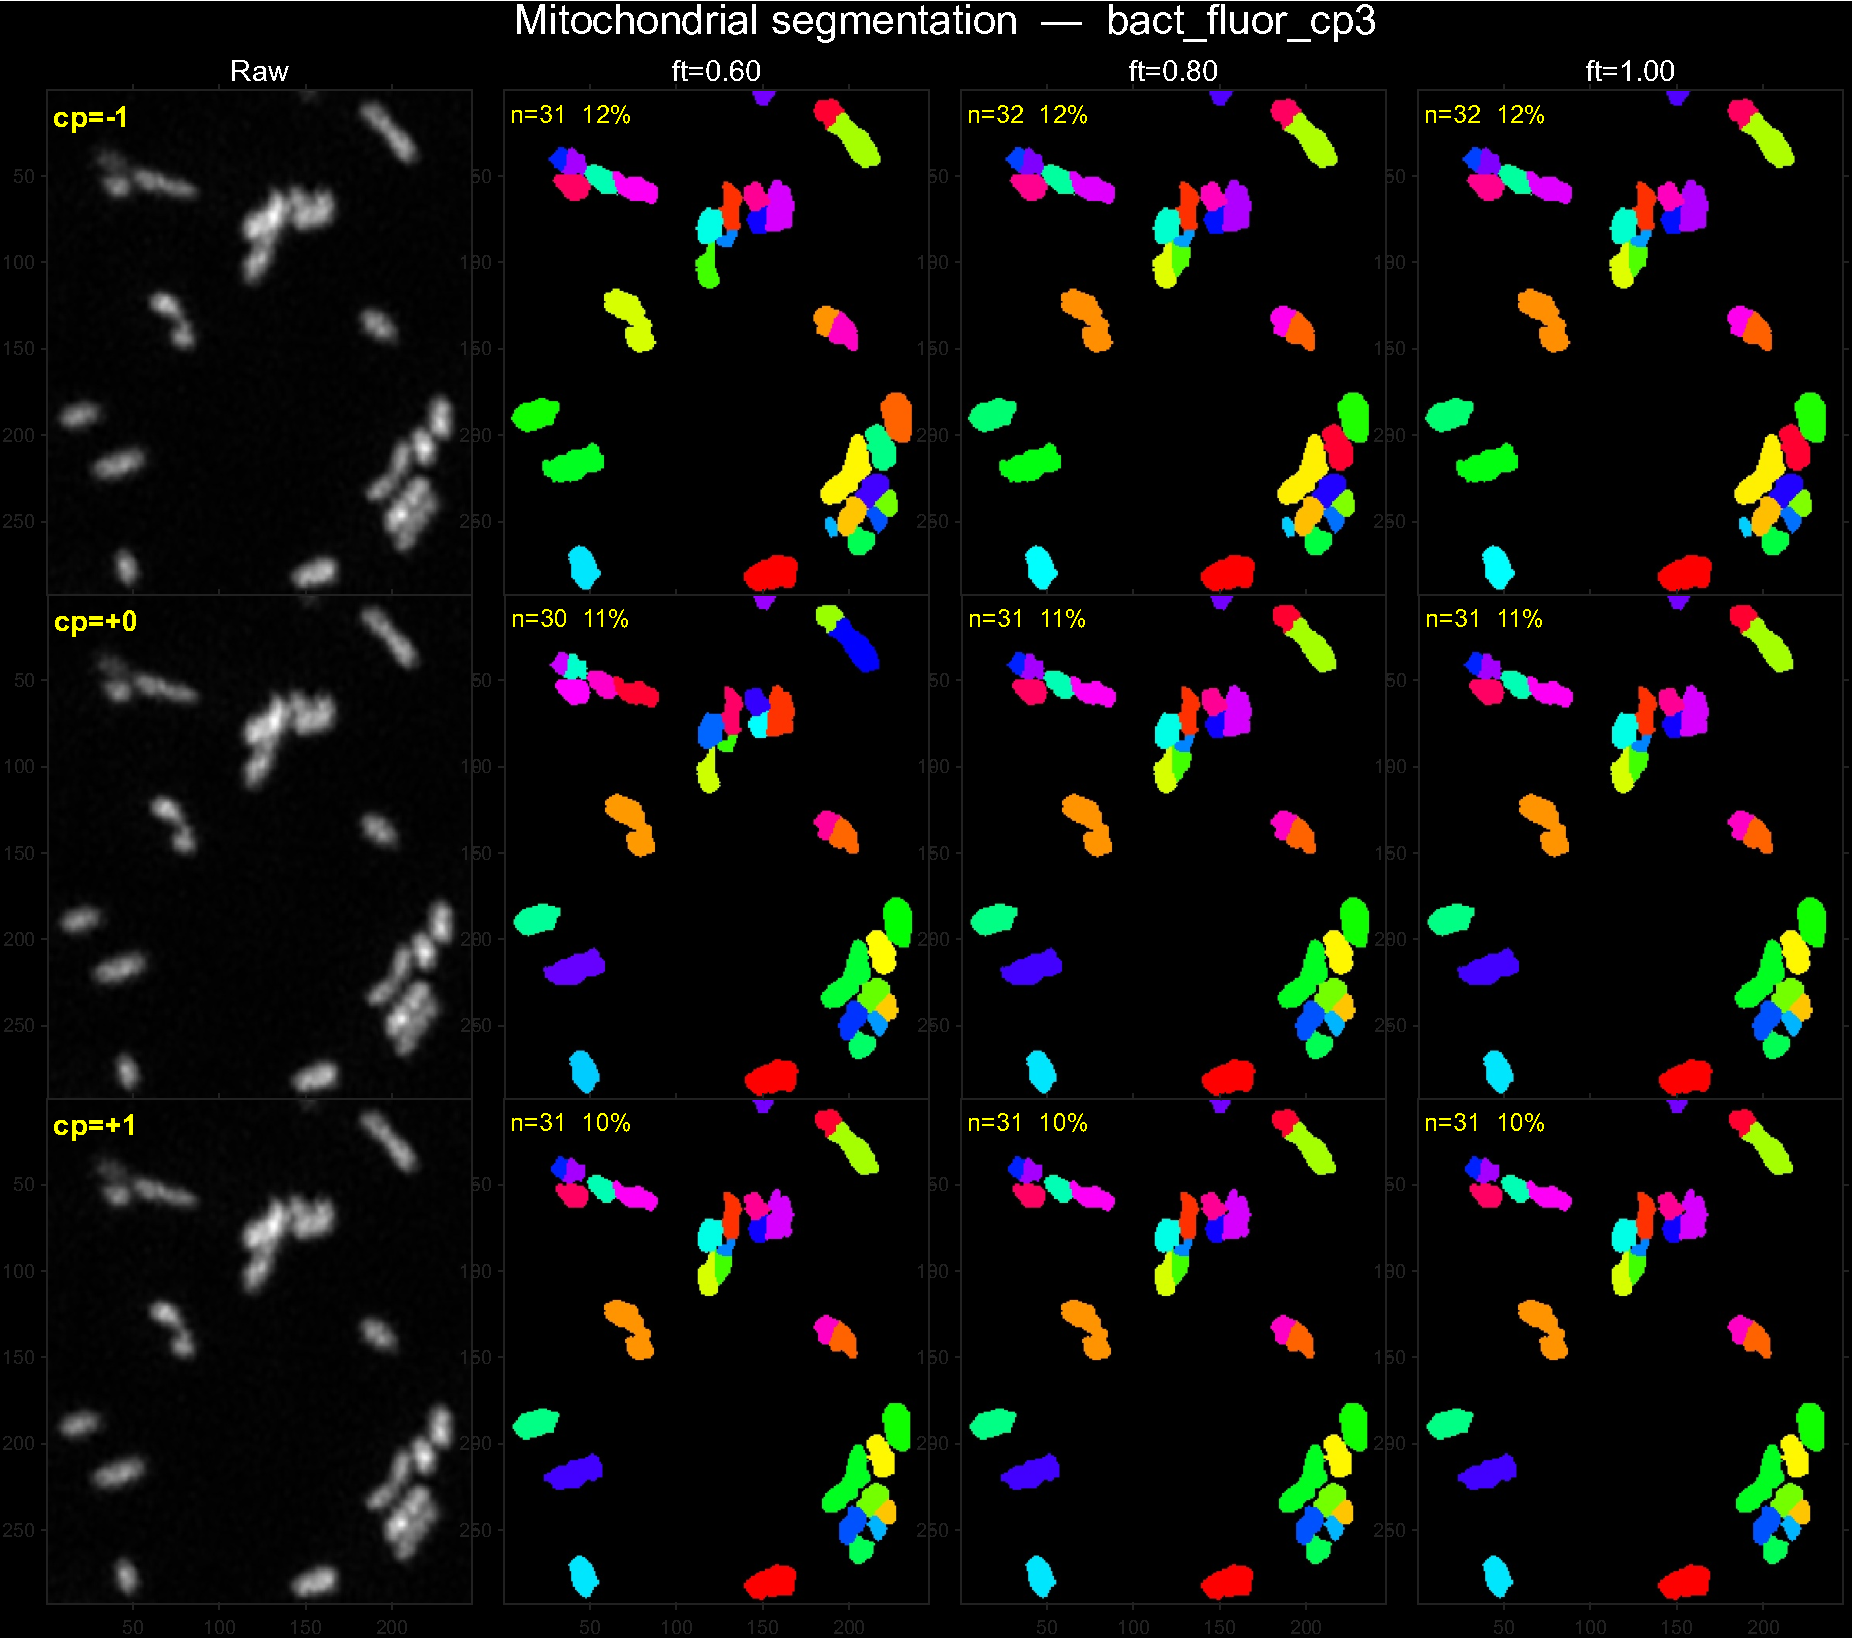
\includegraphics[width=\linewidth]{figures/cellpose_sweep_labels_bact_fluor_cp3.pdf}
  \caption{\texttt{bact\_fluor\_cp3} label grid (default \texttt{nIter}).
    Layout as Figure~\ref{fig:cellpose-cyto3-labels}.}
  \label{fig:cellpose-bact-labels}
\end{figure*}
}{%
\begin{quote}\textit{Run \texttt{sweepCellpose.m} with \texttt{doExport = true}
  to generate \texttt{cellpose\_sweep\_labels\_bact\_fluor\_cp3.pdf}.}\end{quote}
}

% =============================================================================
\chapter{Orientation Analysis and Pre-filtering}
\label{ch:orientation}

% -----------------------------------------------------------------------------
\section{\texttt{structureTensorEnhance}}
\label{sec:st}

\newthought{The structure tensor}~\cite{Bigun1987,Weickert1998} encodes local
image orientation.  The tensor is formed from the outer product of the image
gradient, smoothed at an integration scale:

\begin{equation}
  J = G_{\sigma_i} * \begin{pmatrix} I_x^2 & I_xI_y \\ I_xI_y & I_y^2 \end{pmatrix},
\end{equation}

where $G_{\sigma_i}$ denotes convolution with a Gaussian of standard deviation
$\sigma_i$ (the integration scale).  The eigenvalues $\lambda_1 \geq \lambda_2
\geq 0$ of $J$ satisfy:
\begin{itemize}
  \item $\lambda_1 \approx \lambda_2 \approx 0$: flat region (no edges)
  \item $\lambda_1 \gg \lambda_2 \approx 0$: linear edge (rod or fibre)
  \item $\lambda_1 \approx \lambda_2 \gg 0$: corner or isotropic texture
\end{itemize}

The \emph{coherence index}

\begin{equation}
  C = \left(\frac{\lambda_1 - \lambda_2}{\lambda_1 + \lambda_2}\right)^2
  \;\in [0, 1]
\end{equation}

is $1$ for a perfect linear structure and $0$ for an isotropic region.
Eigenvalues are computed from the analytically stable formula
$\lambda_{1,2} = \tfrac{1}{2}\bigl[(J_{11}+J_{22}) \pm
\sqrt{(J_{11}-J_{22})^2 + 4J_{12}^2}\bigr]$.

The dominant along-fibre orientation (second output \texttt{theta}) is in
$[-\pi/2, \pi/2]$ radians from horizontal.

\subsection*{Usage as a post-weight}

\begin{lstlisting}
pST.sigmaGrad = 1.5; pST.sigmaInt = 5; pST.normalize = true;
[C, theta] = structureTensorEnhance(I, pST);

R_rod    = rodGranulometryEnhance(I) .* C;      % suppress puncta
R_puncta = logEnhance(I)             .* (1-C);  % suppress rods
\end{lstlisting}

\subsection*{Parameters}
\marginnote{%
  \textbf{\texttt{sigmaGrad}} \newline
  Gaussian pre-smoothing before gradient (px). Default \texttt{1.5}.\newline
  Should suppress pixel noise without blurring structure boundaries.
  \medskip\par
  \textbf{\texttt{sigmaInt}} \newline
  Integration scale (px). Default \texttt{5}.\newline
  Should match roughly half the structure width.
  \medskip\par
  \textbf{\texttt{normalize}} Default \texttt{true}.
}

% -----------------------------------------------------------------------------
\section{\texttt{orientedGaussSmooth}}
\label{sec:ogs}

\newthought{Orientation-adaptive smoothing} is a single-pass, non-iterative
approximation to Coherence-Enhancing Diffusion~\cite{Weickert1999}.  The image
is pre-convolved with $N$ Gaussian kernels elongated at discrete orientations
$\theta_k$:

\begin{equation}
  G_k(I) = I * \mathcal{N}\!\left(0,\,
            R_{\theta_k}\,\mathrm{diag}(\sigma_\parallel^2,\sigma_\perp^2)
            \,R_{\theta_k}^\top\right),
\end{equation}

and the outputs are blended per-pixel using cosine-squared weights scaled by
the coherence index:

\begin{equation}
  w_k = C\cos^2\!\left(\theta - \theta_k\right) + \frac{1-C}{N},
  \qquad
  \hat{I} = \frac{\sum_k w_k G_k(I)}{\sum_k w_k}.
\end{equation}

Because $\sum_k \cos^2(\theta-\theta_k) = N/2$ exactly for uniform spacing,
the denominator simplifies to $1 + C(N/2-1)$---no per-pixel loop is required.
Where $C\approx 0$ (puncta, noise, flat regions) the filter reduces to isotropic
averaging with scale $\sigma_\perp$; where $C\approx 1$ it extends
$\sigma_\parallel$ along the fibre with minimal blurring across it.

\subsection*{Parameters}
\marginnote{%
  \textbf{\texttt{sigmaAlong}} \newline
  Along-fibre smoothing (px). Default \texttt{4}.
  \medskip\par
  \textbf{\texttt{sigmaAcross}} \newline
  Across-fibre smoothing (px). Default \texttt{1.5}.\newline
  Keep small to preserve cross-fibre boundaries.
  \medskip\par
  \textbf{\texttt{orientations}} \newline
  Discrete angles in $[0^\circ,180^\circ)$. Default \texttt{8}.
  \medskip\par
  \textbf{\texttt{sigmaGrad}, \texttt{sigmaInt}} \newline
  Internal structure tensor scales. Defaults \texttt{1.5} and \texttt{5}.
}

\begin{lstlisting}
pOGS.sigmaAlong  = 4;   pOGS.sigmaAcross = 1.5;
pOGS.orientations = 8;
Ism = orientedGaussSmooth(I, pOGS);
R   = rodGranulometryEnhance(Ism, pRod);   % enhanced input
\end{lstlisting}

% =============================================================================
\chapter{Demo Scripts}
\label{ch:demos}

\section{\texttt{demoMitoEnhance}}

\newthought{This script} runs all six enhancers on both a synthetic test image
(generated by \texttt{makeMitoTestImage}) and a real confocal image
(\texttt{mitImage.mat}), producing eight figures.

\begin{description}
  \item[Figure~\ref{fig:synth_annotated}] Annotated synthetic test image with
    region labels (isolated rods, clustered rods, two network motifs).
  \item[Figure~\ref{fig:comparison_synth}] Six-panel comparison on the synthetic
    image: raw, LoG, fiberEnhance, capsule single, capsule DoC, granulometry.
  \item[Figure~\ref{fig:comparison_real}] Same six-panel layout on the real
    confocal image.
  \item[Figure 4--6] Additional diagnostic comparisons (DoC vs single,
    granulometry vs LoG).
  \item[Figure~\ref{fig:coherence}] Structure tensor coherence: coherence map
    $C$, DoC$\times C$ (rod channel), and LoG$\times(1-C)$ (puncta channel).
  \item[Figure~\ref{fig:rodvsdisk}] Rod vs disk granulometry: line openings
    suppress puncta that disk openings preserve.
\end{description}

\begin{figure*}
  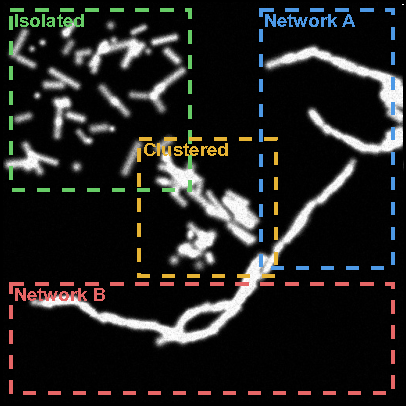
\includegraphics[width=\linewidth]{figures/fig01_synthetic_annotated.pdf}
  \caption{Annotated synthetic test image.  Four region types are highlighted:
    isolated rods (green), clustered rods (amber), two network motifs (blue, red).}
  \label{fig:synth_annotated}
\end{figure*}

\begin{figure*}
  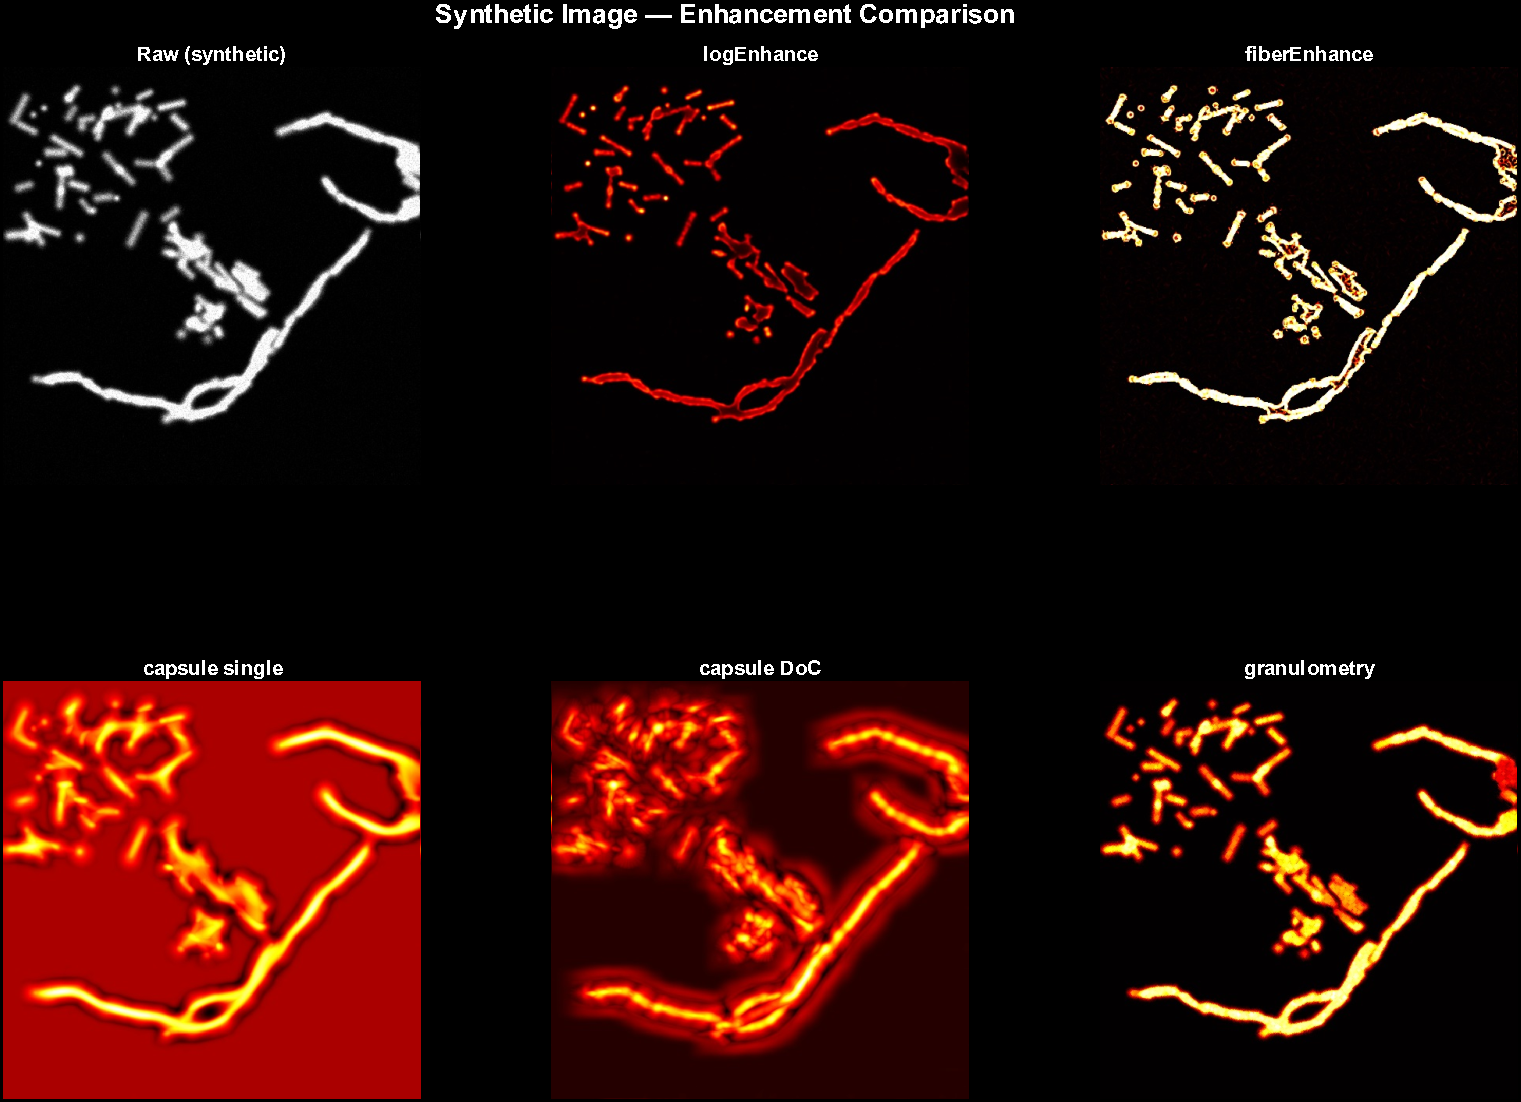
\includegraphics[width=\linewidth]{figures/fig02_comparison_synth.pdf}
  \caption{Enhancement comparison on the synthetic image.  All maps are
    normalised to $[0,1]$ and displayed with the \textit{hot} colourmap.}
  \label{fig:comparison_synth}
\end{figure*}

\begin{figure*}
  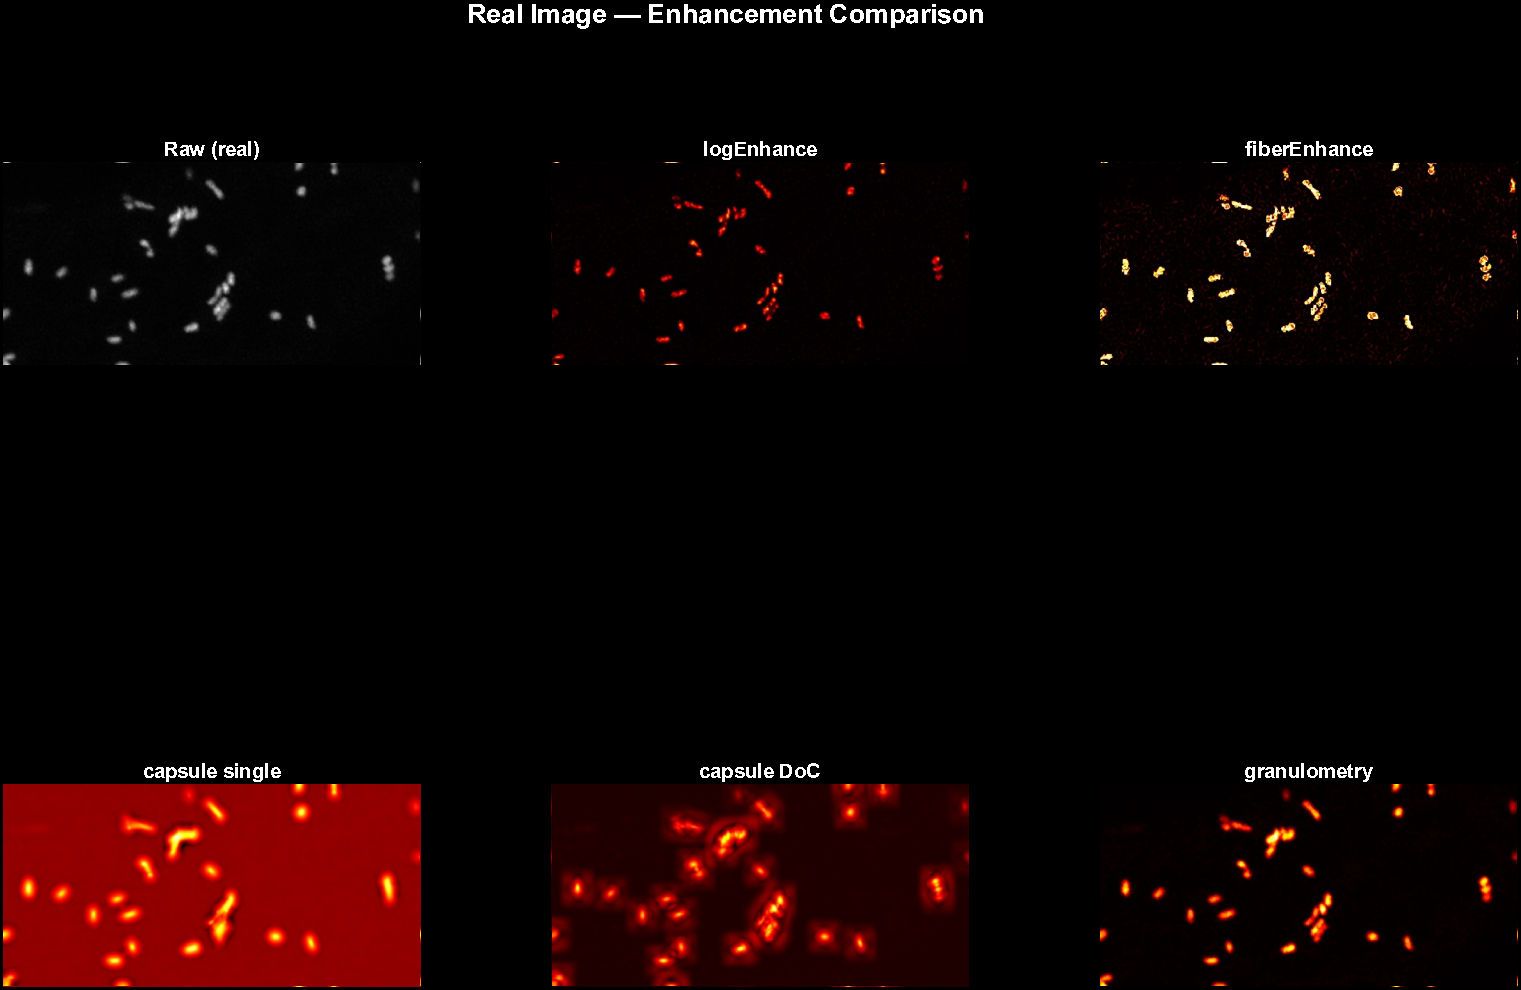
\includegraphics[width=\linewidth]{figures/fig03_comparison_real.pdf}
  \caption{Enhancement comparison on the real confocal image.}
  \label{fig:comparison_real}
\end{figure*}

\begin{figure*}
  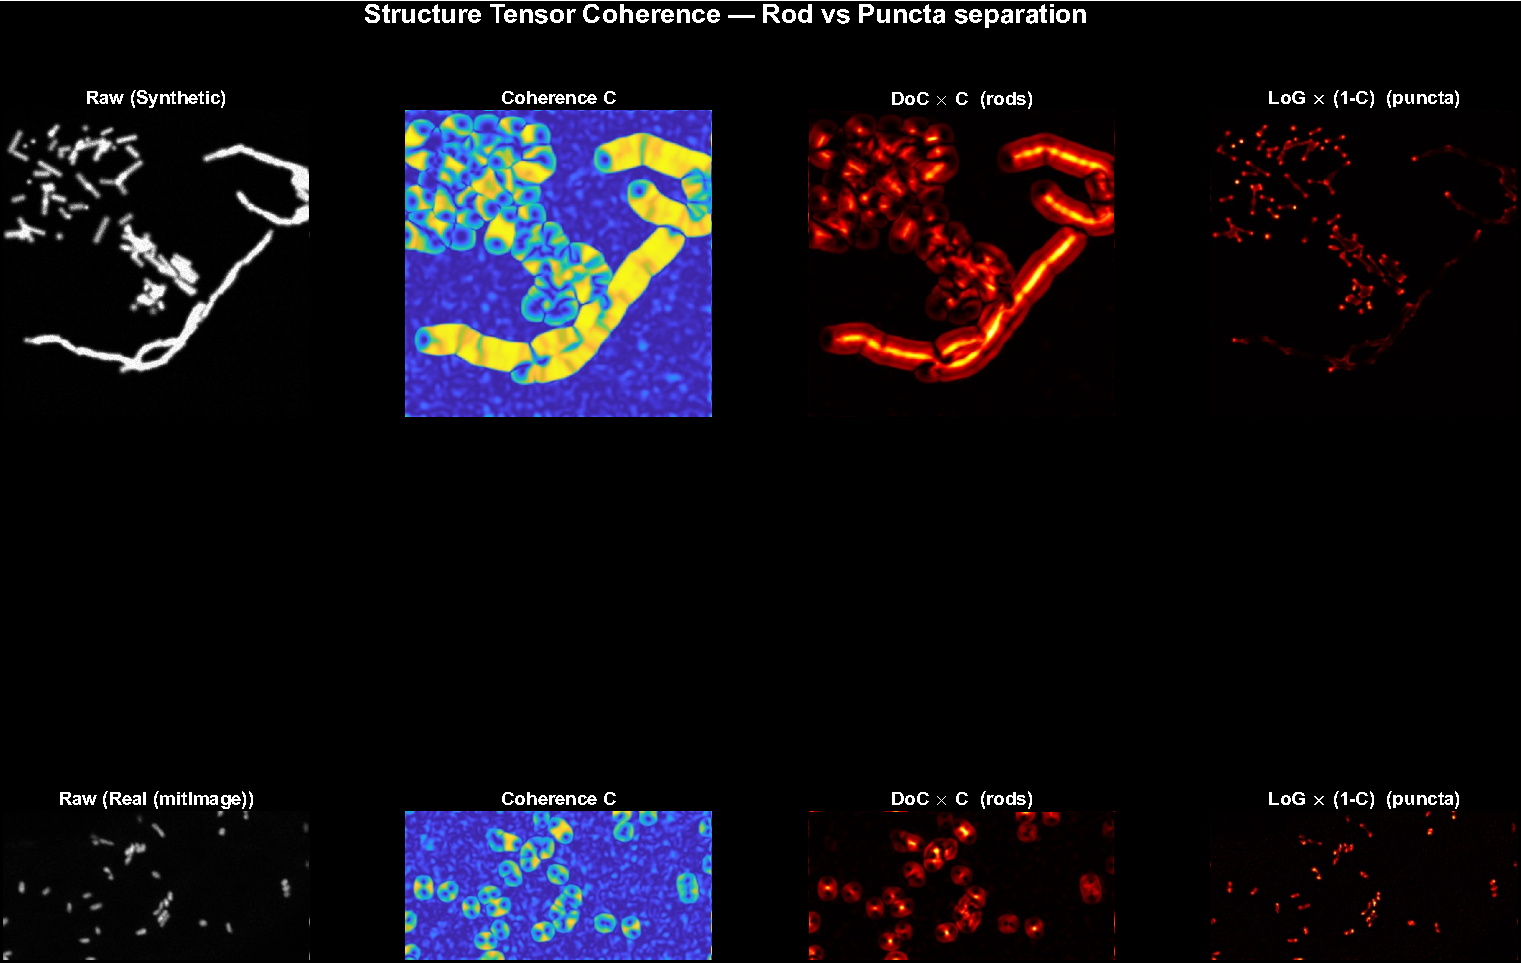
\includegraphics[width=\linewidth]{figures/fig04_coherence_separation.pdf}
  \caption{Structure tensor coherence applied as a multiplicative post-weight.
    Left: coherence map $C$ (\textit{parula} colourmap).  Centre: DoC$\times C$
    (rod channel).  Right: LoG$\times(1-C)$ (puncta channel).}
  \label{fig:coherence}
\end{figure*}

\begin{figure*}
  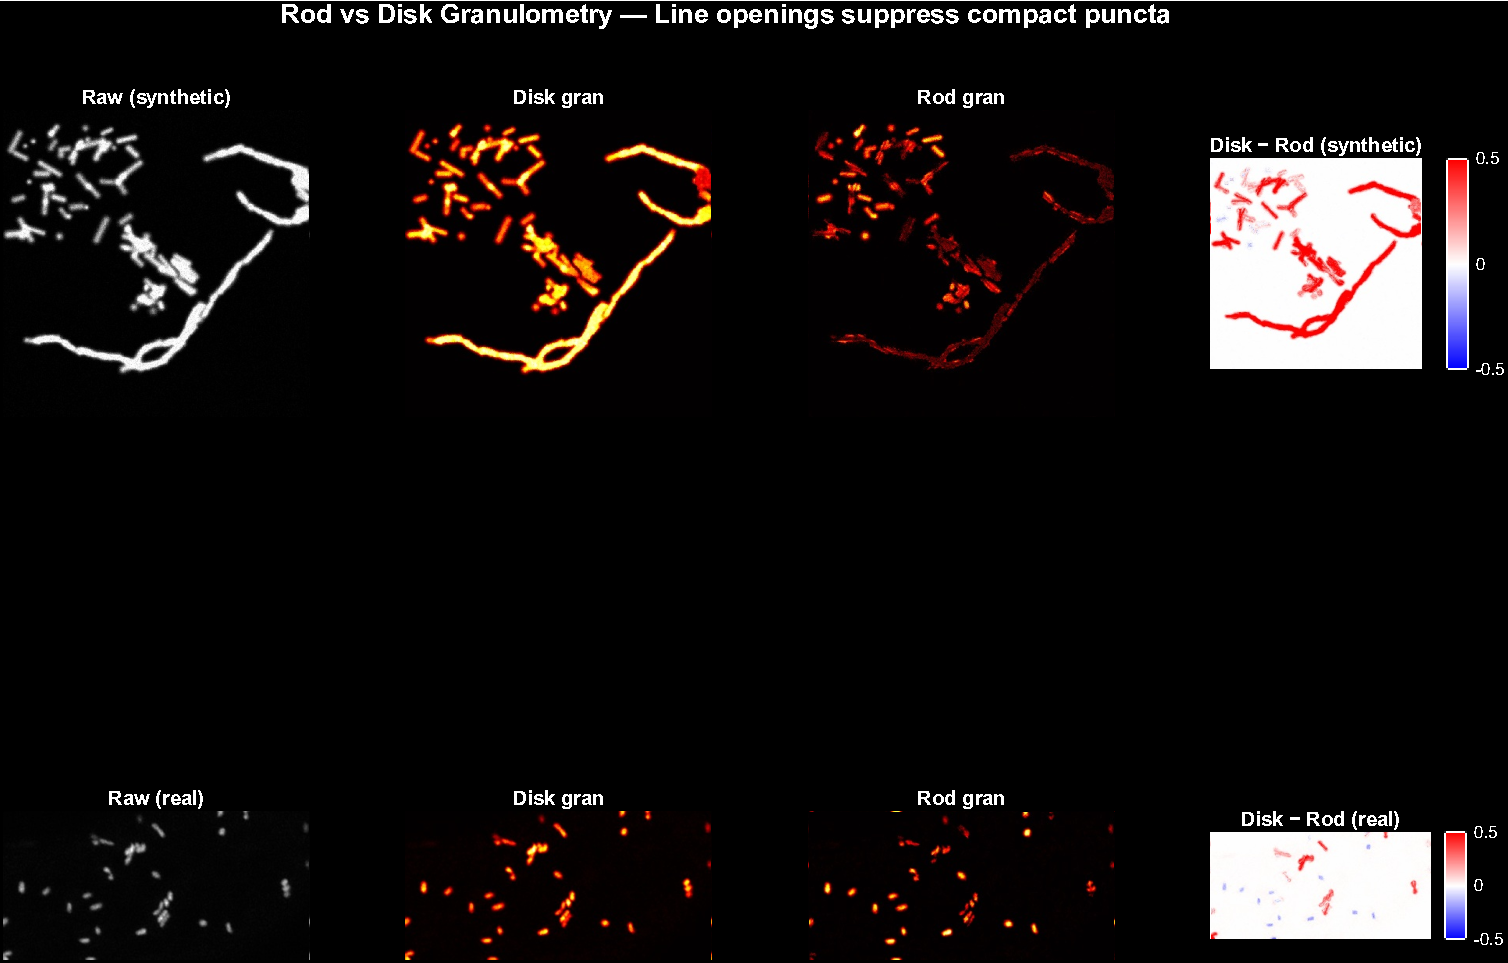
\includegraphics[width=\linewidth]{figures/fig05_rod_vs_disk.pdf}
  \caption{Rod vs disk granulometry.  The difference map (disk$-$rod) reveals
    compact structures that disk openings preserve but line openings suppress.}
  \label{fig:rodvsdisk}
\end{figure*}

% -------------------------------------------------------------------------
\section{\texttt{demoPrefilter}}

\newthought{This script} compares three pre-filtering strategies and their
effect on the two most powerful rod detectors
(Sections~\ref{sec:fiber} and~\ref{sec:rodgran}).  One figure is generated
per method; each is a $2\times3$ panel (rows: synthetic / real; columns:
pre-filtered image, rod granulometry, fiberEnhance).

\begin{description}
  \item[Figure~\ref{fig:pf_raw}] Baseline: no pre-filtering.
  \item[Figure~\ref{fig:pf_pm}] Perona-Malik anisotropic diffusion
    (\texttt{imdiffusefilt}, 15 iterations, threshold 0.03).
    Smooths within regions; stops at intensity edges; not directionally steered.
  \item[Figure~\ref{fig:pf_guided}] Guided filter (\texttt{imguidedfilter},
    neighbourhood 7, regularisation $5\times10^{-3}$).
    Intensity-similarity gated; very fast; not directionally steered.
  \item[Figure~\ref{fig:pf_ogs}] Orientation-adaptive Gaussian smoothing
    (\texttt{orientedGaussSmooth}, $\sigma_\parallel=4$, $\sigma_\perp=1.5$).
    Directionally steered; suppresses cross-fibre noise while preserving
    cross-fibre boundaries.
\end{description}

\begin{figure*}
  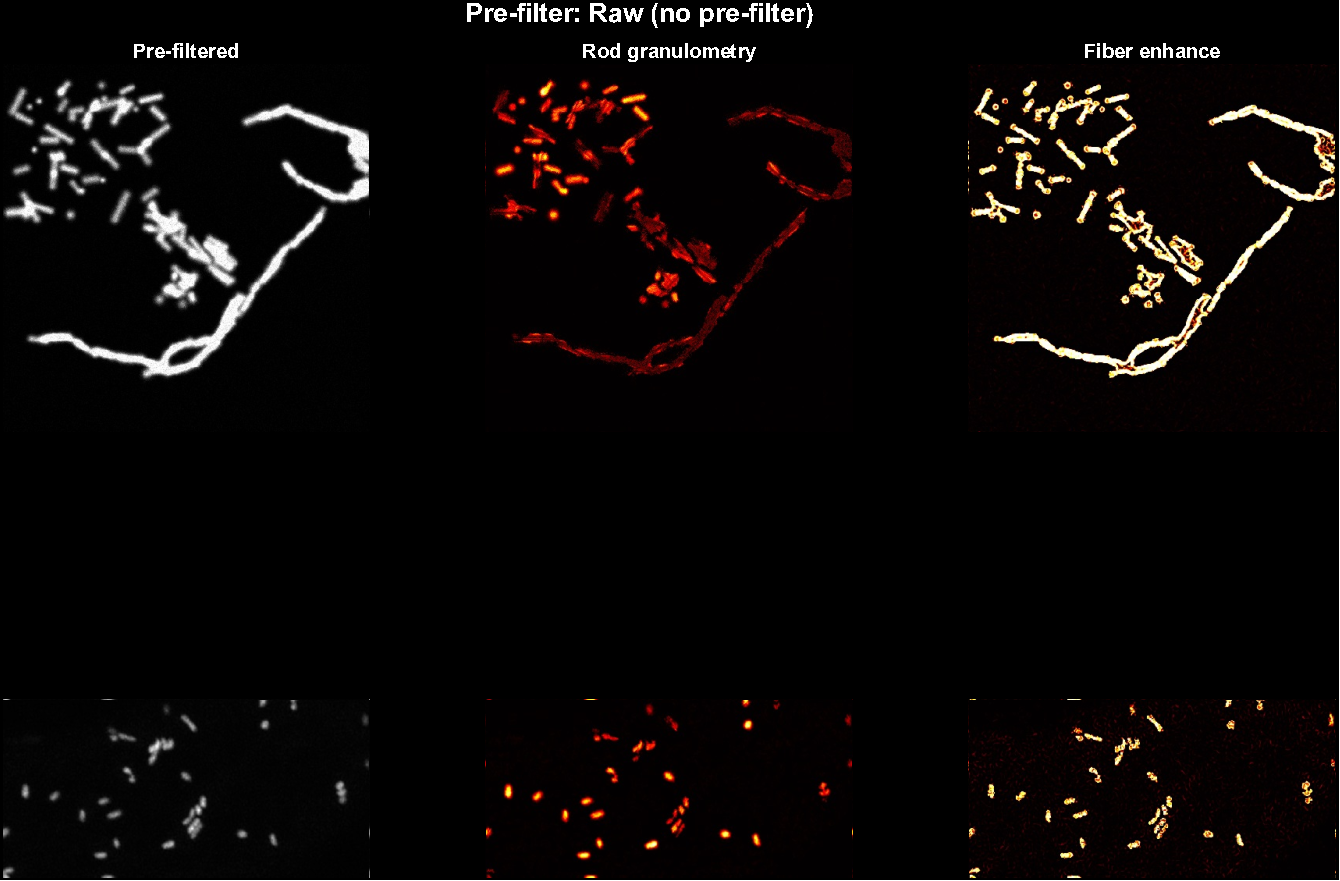
\includegraphics[width=\linewidth]{figures/fig06_prefilter_raw.pdf}
  \caption{Pre-filter baseline (no pre-filtering).  Top row: synthetic image.
    Bottom row: real confocal image.}
  \label{fig:pf_raw}
\end{figure*}

\begin{figure*}
  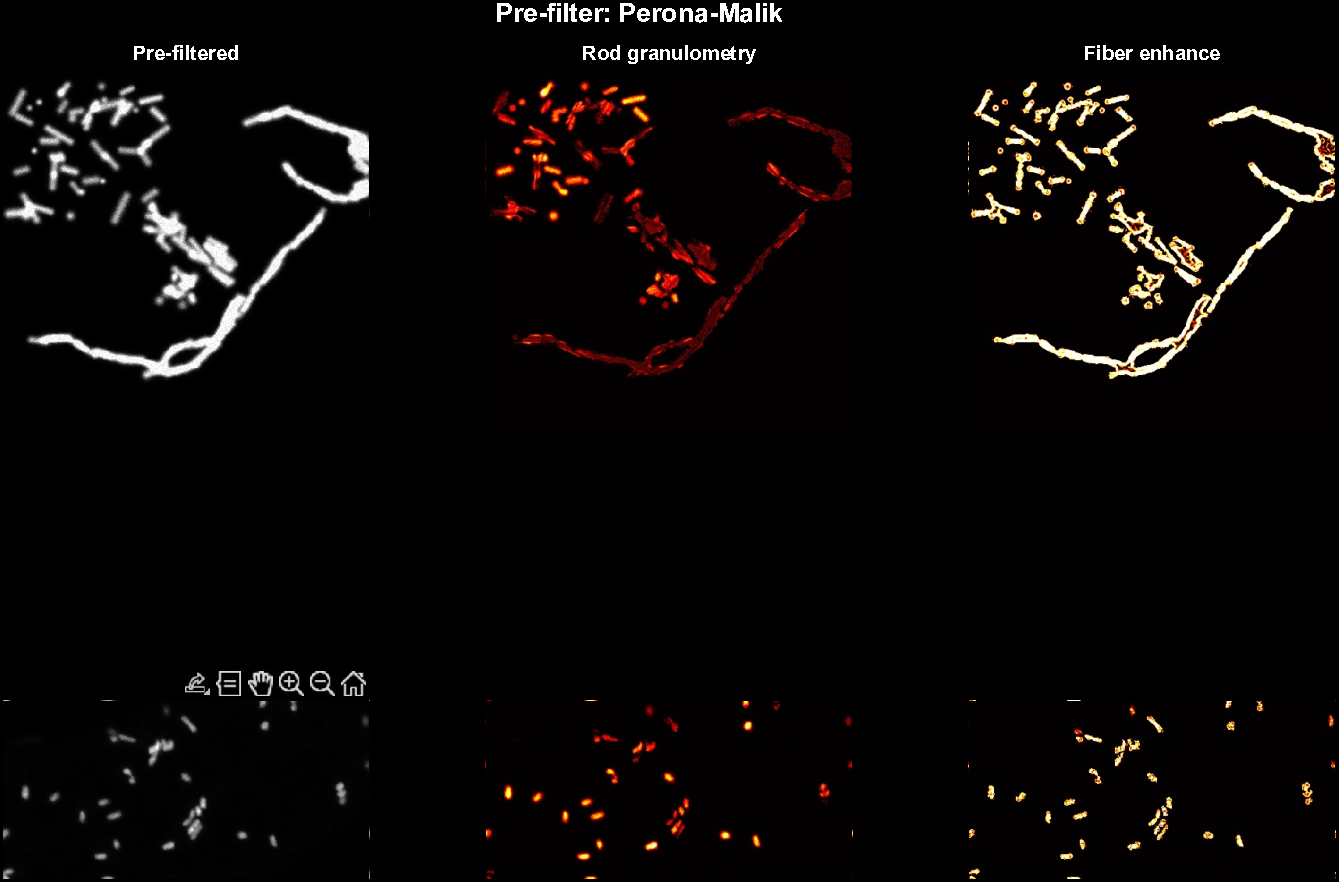
\includegraphics[width=\linewidth]{figures/fig07_prefilter_pm.pdf}
  \caption{Perona-Malik anisotropic diffusion as pre-filter.}
  \label{fig:pf_pm}
\end{figure*}

\begin{figure*}
  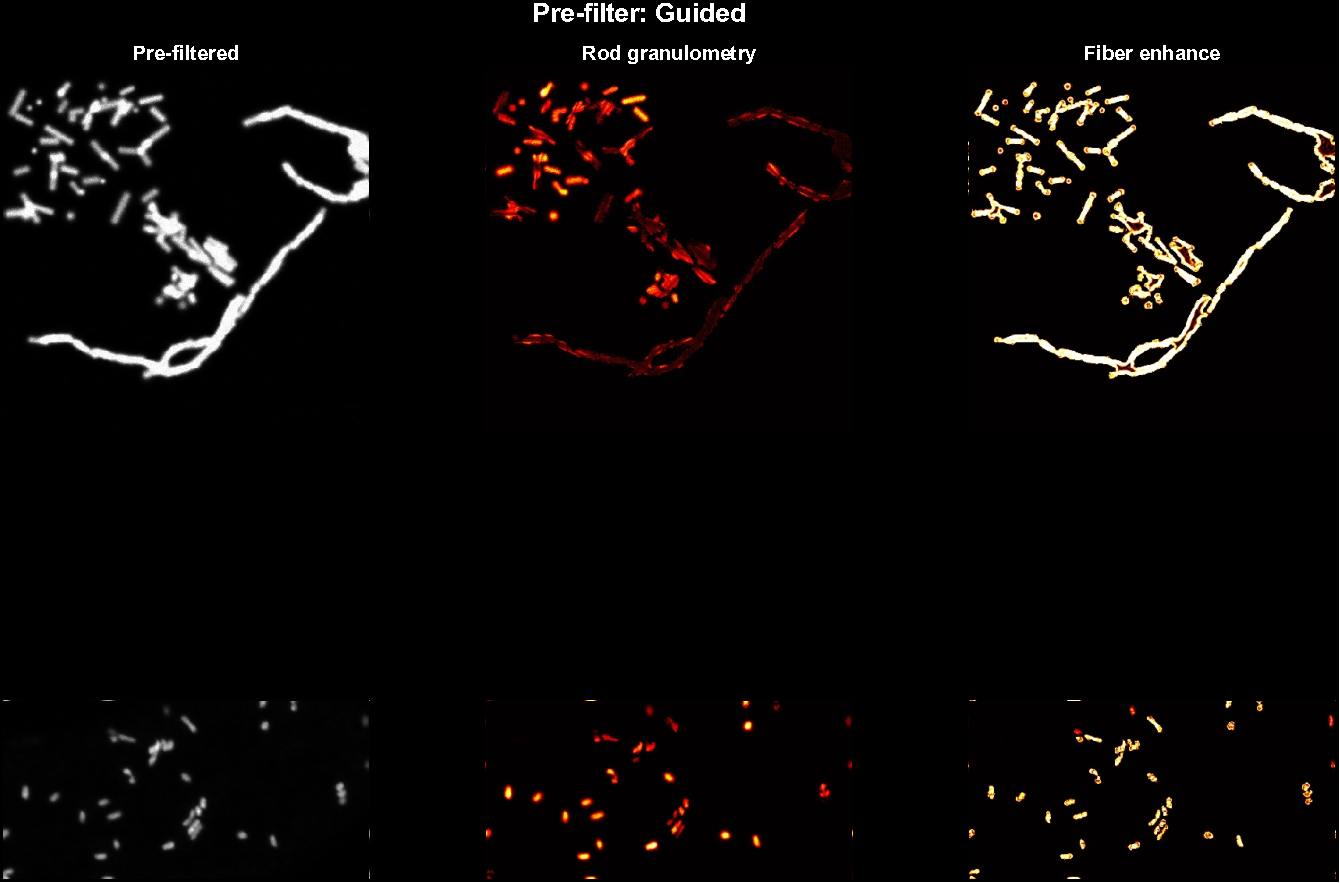
\includegraphics[width=\linewidth]{figures/fig08_prefilter_guided.pdf}
  \caption{Guided filter as pre-filter.}
  \label{fig:pf_guided}
\end{figure*}

\begin{figure*}
  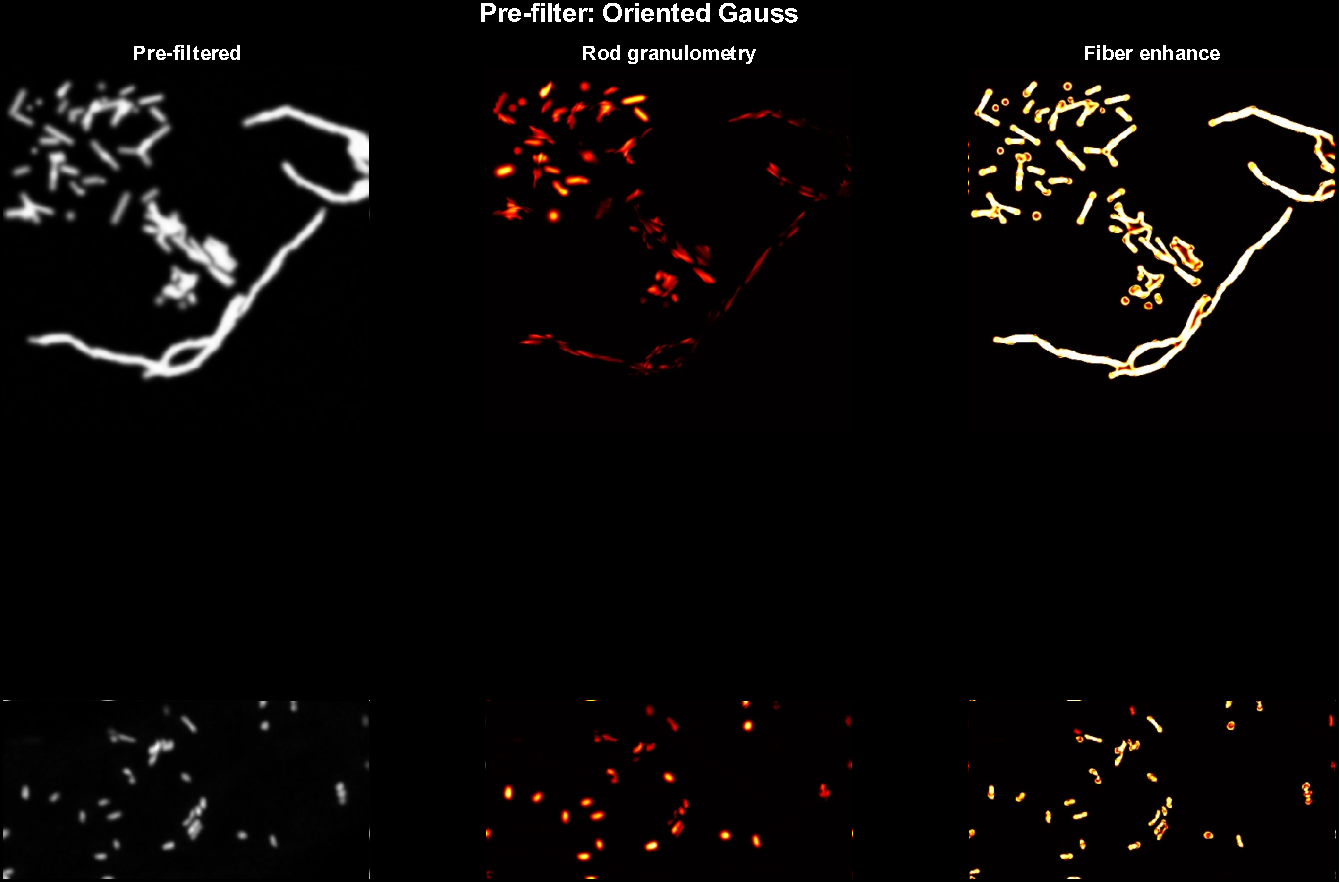
\includegraphics[width=\linewidth]{figures/fig09_prefilter_ogs.pdf}
  \caption{Orientation-adaptive Gaussian smoothing as pre-filter.}
  \label{fig:pf_ogs}
\end{figure*}

% -------------------------------------------------------------------------
\section{\texttt{demoMitoEnhance} --- Cellpose comparison}

When the Cellpose add-on is installed, \texttt{demoMitoEnhance} produces a
ninth figure comparing the \texttt{cyto3} segmentation with the raw image.
Three columns are shown per image row:

\begin{description}
  \item[Raw] Original grayscale image (grey colourmap).
  \item[Binary mask] The $\{0,1\}$ output \texttt{R} from
    \texttt{cellposeEnhance} (\textit{hot} colourmap).
  \item[Instance labels] The \texttt{uint16} label image \texttt{L} rendered
    with \texttt{label2rgb}: each object receives a distinct hue, making
    touching objects visually distinguishable.
\end{description}

\IfFileExists{figures/fig10_cellpose.pdf}{%
\begin{figure*}
  \includegraphics[width=\linewidth]{figures/fig10_cellpose.pdf}
  \caption{Cellpose \texttt{cyto3} segmentation (\texttt{diameter}=10\,px).
    Left: raw image.  Centre: binary detection mask \texttt{R}.
    Right: coloured instance labels \texttt{L} --- touching objects are
    assigned distinct hues.}
  \label{fig:cellpose}
\end{figure*}
}{%
\begin{quote}
  \textit{Figure not available: run \texttt{docs/exportFigures.m} with the
  Cellpose add-on installed to generate \texttt{fig10\_cellpose.pdf}.}
\end{quote}
}

% =============================================================================
\chapter{Unit Tests}
\label{ch:tests}

\newthought{A MATLAB unit test class} \texttt{tests/testBlobFilters.m}
verifies all seven functions using the \texttt{matlab.unittest} framework
introduced in R2013b.  Run the full suite with:

\begin{lstlisting}
results = runtests('tests/testBlobFilters');
table(results)
\end{lstlisting}

The 49 tests cover four categories for each function:

\begin{enumerate}
  \item \textbf{Contract} -- output size matches input; class is
    \texttt{single}; range is $[0,1]$ when \texttt{normalize=true}.
  \item \textbf{Uniform image} -- constant input yields zero (or constant)
    output, confirming that the function does not hallucinate structure.
  \item \textbf{Selectivity} -- response is higher in a known synthetic
    structure than in a background region.
  \item \textbf{Error handling} -- invalid inputs and edge cases raise the
    expected warnings or errors.
\end{enumerate}

% =============================================================================
\chapter*{References}
\addcontentsline{toc}{chapter}{References}

\begin{thebibliography}{99}

\bibitem{Stringer2021}
Stringer~C., Wang~T., Michaelos~M. \& Pachitariu~M. (2021)
Cellpose: a generalist algorithm for cellular segmentation.
\textit{Nature Methods} \textbf{18}:100--106.
\url{https://doi.org/10.1038/s41592-020-01018-x}

\bibitem{Pachitariu2022}
Pachitariu~M. \& Stringer~C. (2022)
Cellpose 2.0: how to train your own model.
\textit{Nature Methods} \textbf{19}:1634--1641.
\url{https://doi.org/10.1038/s41592-022-01663-4}

\bibitem{Stringer2025}
Stringer~C. \& Pachitariu~M. (2025)
Cellpose3: one-click image restoration for improved cellular segmentation.
\textit{Nature Methods} \textbf{22}:592--599.
\url{https://doi.org/10.1038/s41592-025-02595-5}

\bibitem{Bigun1987}
Bigun~J. \& Granlund~G.H. (1987)
Optimal orientation detection of linear symmetry.
\textit{Proc.\ 1st IEEE ICCV}, pp.~433--438.

\bibitem{Frangi1998}
Frangi~A.F., Niessen~W.J., Vincken~K.L. \& Viergever~M.A. (1998)
Multiscale vessel enhancement filtering.
In: Wells W.M. \textit{et al.} (eds) \textit{MICCAI 1998},
LNCS~1496, pp.~130--137. Springer, Berlin.
\url{https://doi.org/10.1007/BFb0056195}

\bibitem{Freeman1991}
Freeman~W.T. \& Adelson~E.H. (1991)
The design and use of steerable filters.
\textit{IEEE Trans.\ Pattern Anal.\ Mach.\ Intell.} \textbf{13}(9):891--906.

\bibitem{Lindeberg1994}
Lindeberg~T. (1994)
\textit{Scale-Space Theory in Computer Vision}.
Kluwer Academic Publishers, Dordrecht.

\bibitem{Lindeberg1998}
Lindeberg~T. (1998)
Feature detection with automatic scale selection.
\textit{Int.\ J.\ Comput.\ Vis.} \textbf{30}(2):79--116.

\bibitem{Maragos1989}
Maragos~P. (1989)
Pattern spectrum and multiscale shape representation.
\textit{IEEE Trans.\ Pattern Anal.\ Mach.\ Intell.} \textbf{11}(7):701--716.

\bibitem{Marr1980}
Marr~D. \& Hildreth~E. (1980)
Theory of edge detection.
\textit{Proc.\ R.\ Soc.\ Lond.\ B} \textbf{207}:187--217.

\bibitem{Serra1982}
Serra~J. (1982)
\textit{Image Analysis and Mathematical Morphology}.
Academic Press, London.

\bibitem{Soille2003}
Soille~P. (2003)
\textit{Morphological Image Analysis}, 2nd edn.
Springer, Berlin.

\bibitem{Weickert1998}
Weickert~J. (1998)
\textit{Anisotropic Diffusion in Image Processing}.
Teubner, Stuttgart.

\bibitem{Weickert1999}
Weickert~J. (1999)
Coherence-enhancing diffusion filtering.
\textit{Int.\ J.\ Comput.\ Vis.} \textbf{31}(2--3):111--127.

\end{thebibliography}

\end{document}
